\documentclass[conference]{IEEEtran}

\usepackage{cite}
\usepackage{amsmath,amssymb}
\usepackage{graphicx}
\usepackage{booktabs}
\usepackage{multirow}
\usepackage{array}
\usepackage{url}

\title{Federated Learning for Massive MIMO Channel Estimation Under IID and Non-IID Client Data}

\author{\IEEEauthorblockN{Anonymous Authors}
\IEEEauthorblockA{Anonymous Institution\\
Email: anonymous@domain.com}}

\begin{document}

\maketitle

\begin{abstract}
Wireless channel estimation has recently benefited from deep learning due to its robustness and low online inference complexity. However, most existing approaches rely on centralized learning, where user-side training data must be collected at a base station, leading to significant communication overhead and limited data privacy. To address this challenge, we develop a federated learning framework for channel estimation in massive MIMO settings, where models are trained across distributed clients without sharing raw channel data. The proposed study evaluates both convolutional and encoder-decoder architectures under centralized and federated protocols, with explicit analysis of IID and non-IID client distributions and FedAvg/FedProx optimization. We further establish a reproducible experimental pipeline with structured run-level logging, statistical summaries, and publication-grade evidence generation. Results indicate that federated learning can achieve competitive estimation performance relative to centralized baselines while exposing clear trade-offs among heterogeneity robustness, communication cost, and architecture choice. These findings support federated channel estimation as a practical direction for privacy-aware and communication-efficient wireless intelligence.
\end{abstract}

\begin{IEEEkeywords}
Federated learning, massive MIMO, channel estimation, non-IID data, FedAvg, FedProx, reproducibility.
\end{IEEEkeywords}

\section{Introduction}
Massive MIMO channel estimation is a foundational signal processing task for modern wireless systems. Recent learning-based estimators outperform classical heuristics in many operating regimes, but they are predominantly trained under centralized learning (CL), where user-side data must be uploaded to a server. This introduces communication overhead and privacy concerns that can become bottlenecks in distributed deployments.

Federated learning (FL) addresses this issue by training global models from local client updates without sharing raw data. However, FL performance is sensitive to client heterogeneity, particularly under non-identically distributed (Non-IID) data partitions. For wireless channel estimation, this creates a practical question: how much estimation quality can be retained under realistic heterogeneous client data while preserving communication and privacy benefits.

This paper presents a systematic and reproducible benchmark study of FL channel estimation under IID and Non-IID client distributions. We compare FedAvg and FedProx using CNN as the primary model and ResUNet as cross-architecture validation. Unlike algorithm-proposal papers, our contribution is a research-grade evaluation protocol with structured run logging, explicit claim-evidence mapping, and publication-ready analysis.

\subsection{Contributions}
\begin{itemize}
    \item A reproducible FL benchmark pipeline for channel estimation with raw-to-paper traceability.
    \item Controlled IID/Non-IID analysis under FedAvg and FedProx protocols.
    \item Cross-architecture validation (CNN primary, ResUNet add-on) for trend consistency.
    \item Quantitative communication-runtime-model-size analysis for deployment relevance.
\end{itemize}

\section{Related Work}
FedAvg introduced communication-efficient decentralized optimization and established a practical FL baseline~\cite{mcmahan2017fedavg}. FedProx extended this framework with proximal regularization for heterogeneous clients~\cite{li2020fedprox}. In wireless systems, Elbir and Coleri demonstrated FL channel estimation in conventional and RIS-assisted massive MIMO, showing promising overhead-performance trade-offs~\cite{elbir2021flchannel}. 

Our work complements these studies by providing a high-coverage benchmark with detailed heterogeneity analysis, reproducible logging, and architecture-level validation across CNN and ResUNet.

\section{System Model and Problem Formulation}
Let $H\in\mathbb{C}^{N_t\times N_s}$ denote the clean channel response and $\tilde H$ the noisy observation from pilot-based acquisition. The estimator outputs $\hat H=f_\theta(\tilde H)$. Performance is measured by normalized mean squared error (NMSE):
\begin{equation}
\mathrm{NMSE}_{\mathrm{dB}} = 10\log_{10}\left(\frac{\|H-\hat H\|_2^2}{\|H\|_2^2}\right).
\end{equation}

In CL, all training samples are centrally aggregated. In FL, each client $k$ trains locally and sends model updates to server. FedAvg aggregation is:
\begin{equation}
\theta^{t+1} = \sum_{k=1}^{K} \frac{n_k}{\sum_j n_j}\theta_k^t,
\end{equation}
where $n_k$ is local dataset size. FedProx solves per-client local objective:
\begin{equation}
\min_{\theta_k} F_k(\theta_k) + \frac{\mu}{2}\|\theta_k-\theta^t\|_2^2.
\end{equation}

\section{Methodology and Reproducibility Protocol}
\subsection{Dataset Construction}
The dataset is generated from DeepMIMO O1\_60. We select 6000 users from BS-0, configure an 8$\times$8 BS array, 1$\times$1 UE array, and 64 OFDM subcarriers. AWGN is injected at SNR levels \{0,5,10,15,20\} dB with per-sample power normalization and fixed RNG seed (42). Complex channels are also stored in real/imaginary stacked format.

For supervised learning, noisy inputs and clean labels are globally normalized, shuffled with fixed seed, and split into 80/20 train/test per SNR.

\subsection{Models}
\textbf{CNN:} lightweight residual denoiser with 19,778 trainable parameters. 
\textbf{ResUNet:} encoder-decoder with skip connections and residual bottleneck, 763,234 parameters.

\subsection{IID and Non-IID Definitions}
IID partitions are generated by global shuffle and uniform client split.

For Non-IID, we use reproducible client-level distribution skew. In ResUNet FL, client dataset is explicitly formed as
\begin{equation}
\mathcal{D}_k=\mathcal{D}_k^u \cup \mathcal{D}_k^s,\quad \rho=\frac{|\mathcal{D}_k^u|}{|\mathcal{D}_k|},
\end{equation}
with $\rho=0.6$ unique norm-sorted segment and 0.4 shared global segment. In CNN FL, Non-IID client sets are generated by dedicated split scripts that induce structured per-client skew before training.

\subsection{Experiment Logging}
Each run logs run ID, hyperparameters, seed, device, per-round/epoch history, and final metrics to JSON/CSV. Federated scripts support checkpoint-resume for long sweeps.

\section{Experimental Setup}
\subsection{Primary CNN Benchmark}
Primary publication benchmark uses 10 dB SNR with:
\begin{itemize}
    \item Centralized CNN: 3 seeds
    \item FedAvg-IID: $R\in\{10,20,30,50\}$, $E\in\{1,2,3,5\}$, 3 seeds
    \item FedAvg-Non-IID: same $R,E$, 3 seeds
    \item FedProx-Non-IID: same $R,E$, $\mu\in\{0.001,0.005,0.01\}$, 3 seeds
\end{itemize}

\subsection{ResUNet Add-on Validation}
A 20-run protocol is used for architecture consistency:
\begin{itemize}
    \item Centralized: 5 seeds
    \item FedAvg-IID: 5 seeds
    \item FedAvg-Non-IID: 5 seeds
    \item FedProx-Non-IID ($\mu=0.001$): 5 seeds
\end{itemize}

\subsection{Classical Baseline}
Least Squares (LS) at 10 dB is included for classical reference. MMSE is discussed but not reported due to missing pilot/covariance calibration in this reproducible pipeline version.

\section{Results and Structured Analysis}
This section follows a consistent pattern: \textit{purpose, observation, interpretation, implication}.

\subsection{Centralized and Federated Performance Summary}
\textbf{Purpose:} establish the global performance landscape before detailed drill-down.

Table~\ref{tab:cnn_stats} summarizes CNN aggregate statistics. The mean ordering indicates heterogeneity penalty from IID to Non-IID and quantifies the trade-off between centralized and federated settings under fixed 10 dB conditions.

\begin{table}[t]
\caption{CNN Statistical Summary at 10 dB}
\label{tab:cnn_stats}
\centering
\begin{tabular}{lcccc}
\toprule
Setting & N & Mean (dB) & Std (dB) & vs CL (dB) \\
\midrule
Centralized & 3 & -19.4227 & 0.1617 & 0.0000 \\
FedAvg-IID & 48 & -19.1190 & 0.6087 & +0.3036 \\
FedAvg-Non-IID & 48 & -18.8483 & 0.5734 & +0.5743 \\
FedProx-Non-IID & 144 & -18.5683 & 0.5498 & +0.8544 \\
\bottomrule
\end{tabular}
\end{table}

\textbf{Observation:} best CNN run (FedAvg-IID) reaches -20.0381 dB, outperforming best centralized seed (-19.6215 dB). At mean level, centralized is -19.4227 dB and FedAvg-IID is -19.1190 dB, i.e., +0.3036 dB gap relative to centralized. FedAvg-Non-IID and FedProx-Non-IID further degrade to -18.8483 dB and -18.5683 dB, respectively.

\textbf{Interpretation:} under aggregate statistics, federated accuracy is competitive but sensitive to data heterogeneity. The best-run advantage of FedAvg-IID indicates that properly tuned federated protocols can match or exceed centralized baselines in specific configurations, while mean-level results require conservative interpretation.

\textbf{Implication:} deployment decisions should rely on both best and mean metrics: best for potential capability, mean/std for operational reliability.

\begin{figure}[t]
\centering
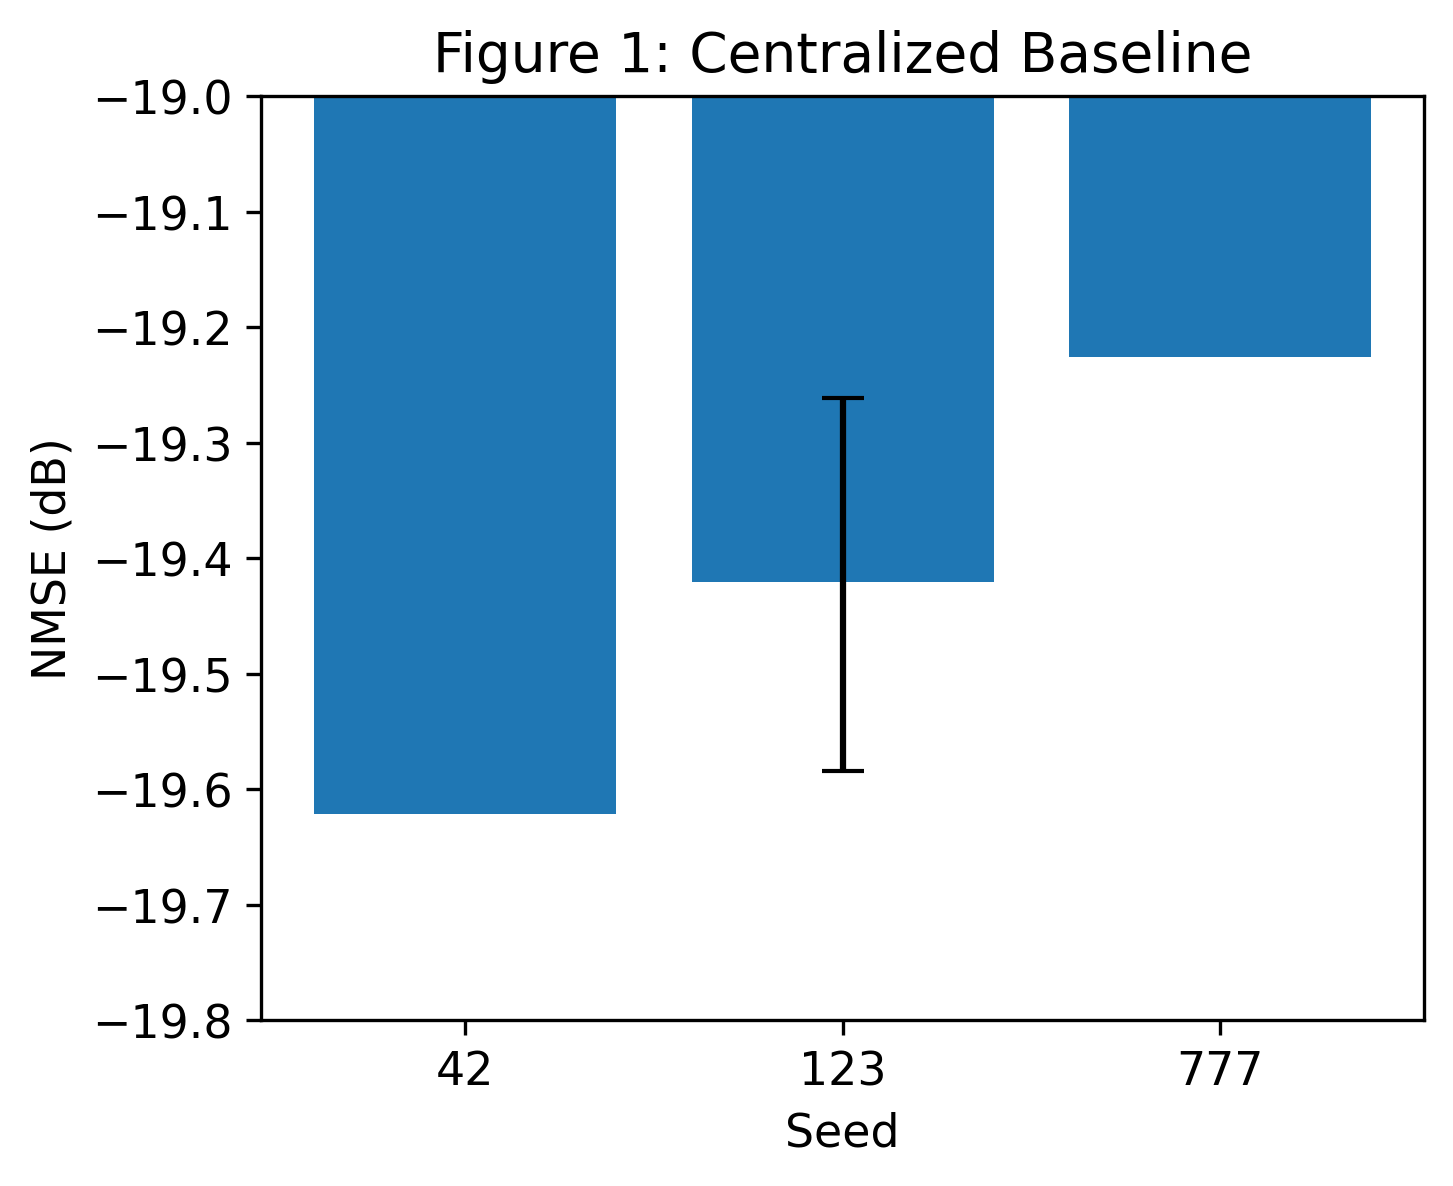
\includegraphics[width=\columnwidth]{results/figures/paper/figure1_centralized_baseline.png}
\caption{Centralized baseline reproducibility across seeds (purpose: CL reference stability).}
\label{fig:f1}
\end{figure}

\subsection{Convergence and Hyperparameter Effects}
\textbf{Purpose:} evaluate how optimization horizon (global rounds) and local compute budget (local epochs) determine final estimation quality.

\begin{figure}[t]
\centering
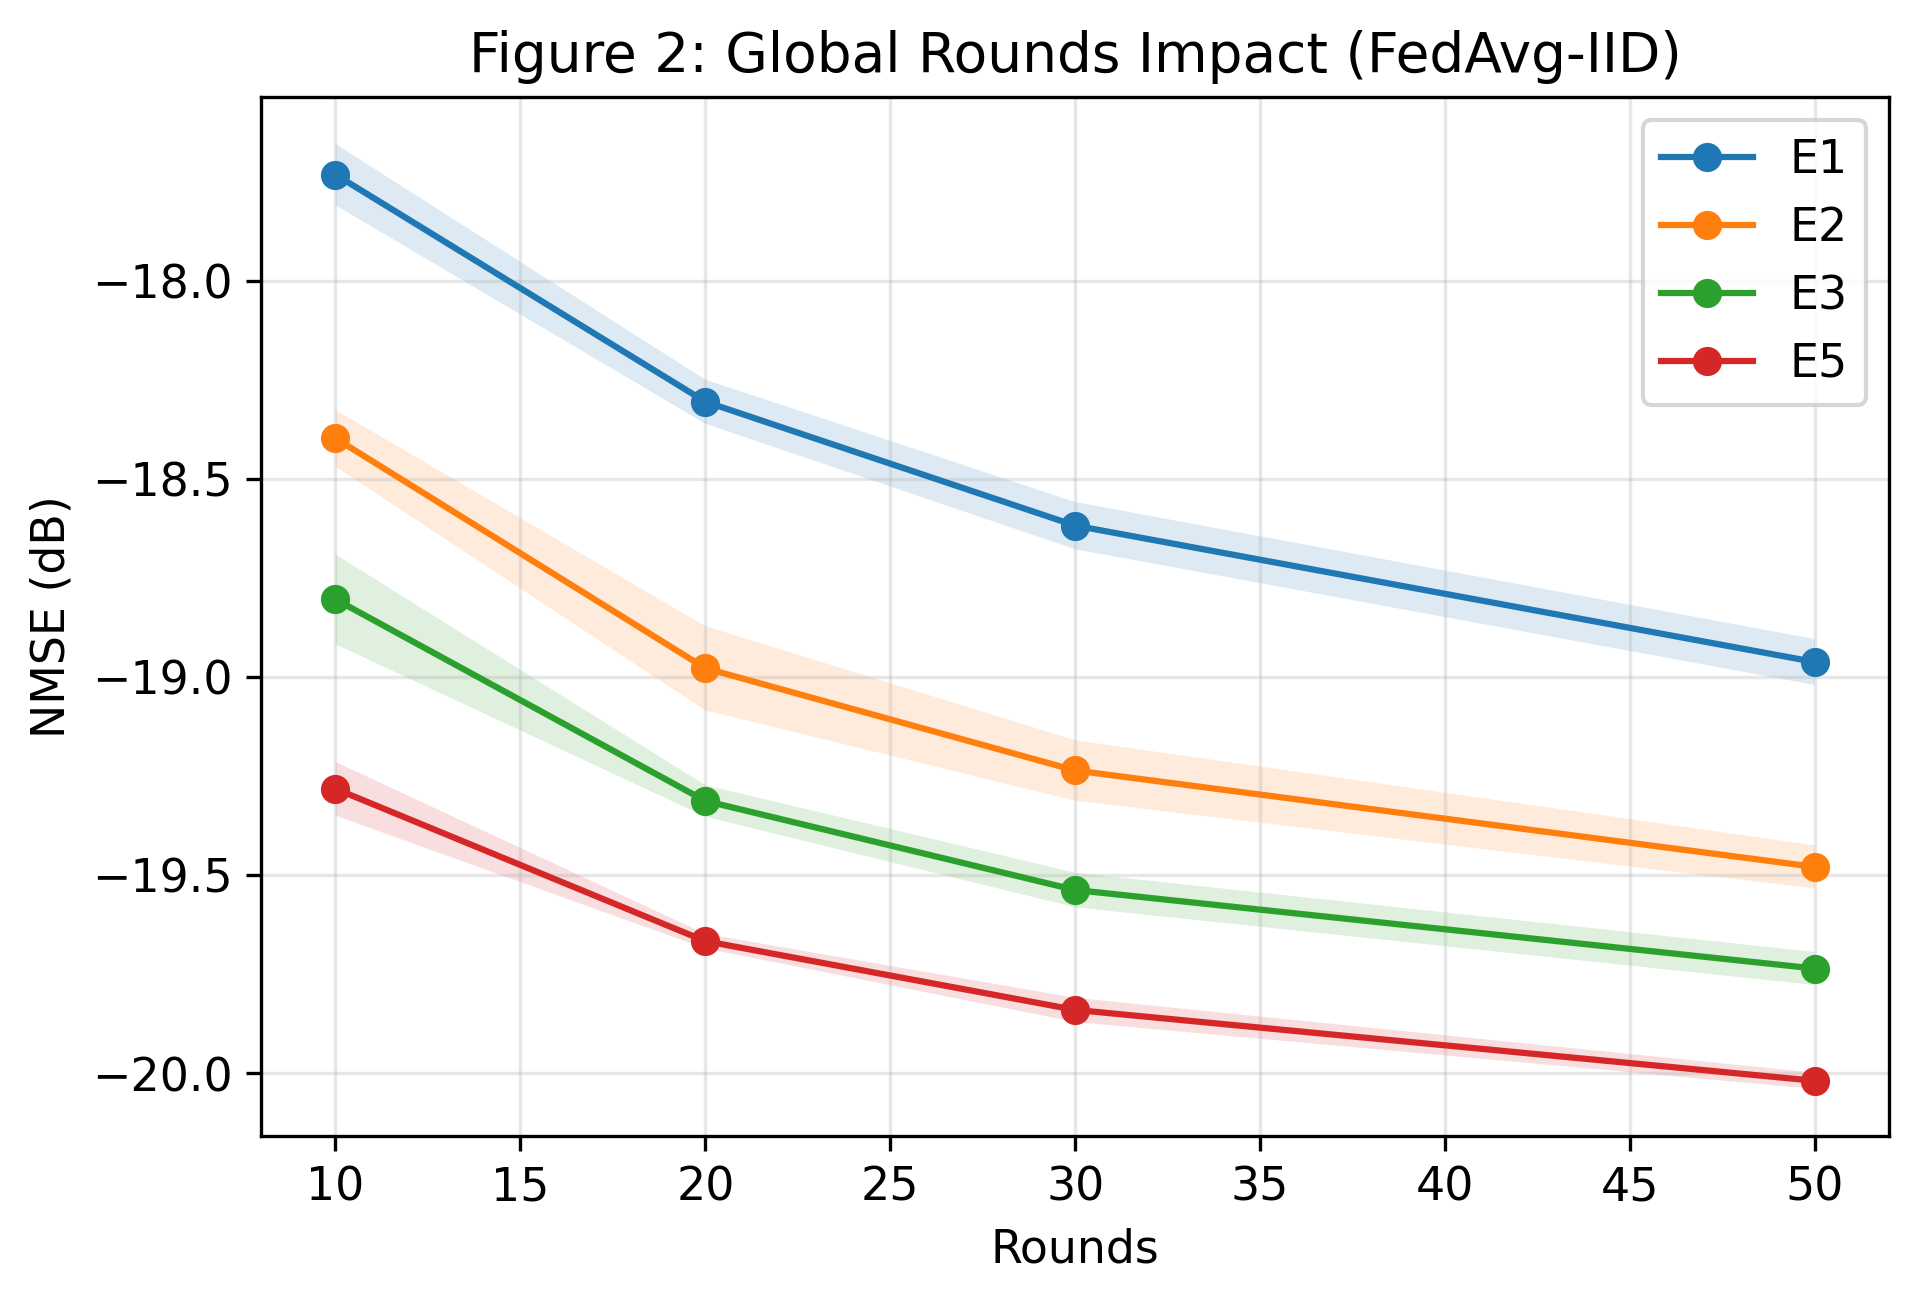
\includegraphics[width=\columnwidth]{results/figures/paper/figure2_rounds_impact_fedavg_iid.png}
\caption{FedAvg-IID rounds impact (purpose: convergence slope and diminishing return region).}
\label{fig:f2}
\end{figure}

\begin{figure}[t]
\centering
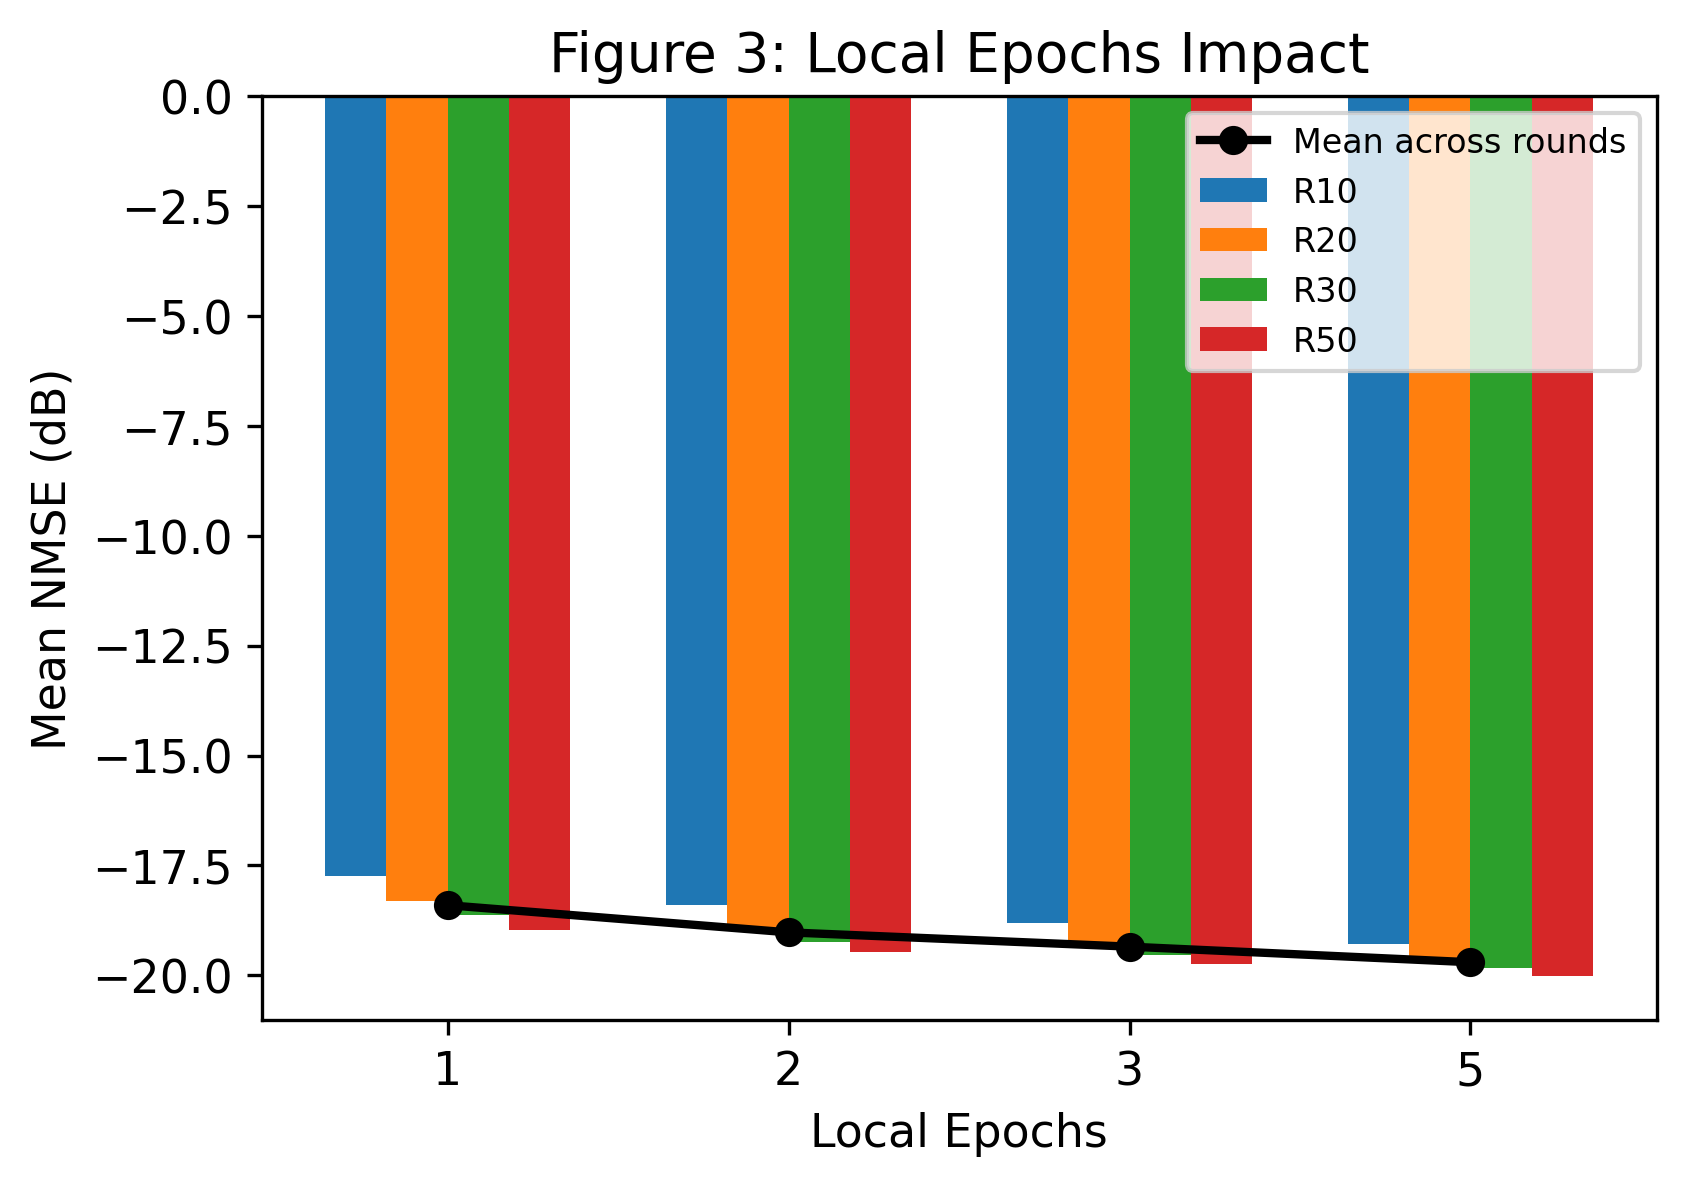
\includegraphics[width=\columnwidth]{results/figures/paper/figure3_local_epochs_impact.png}
\caption{Local epochs impact (purpose: local computation vs global convergence quality).}
\label{fig:f3}
\end{figure}

\textbf{Observation:} increasing rounds and local epochs consistently improves NMSE in IID settings. From low-budget to high-budget configurations, accuracy gains are substantial at early scaling and gradually saturate at larger round counts.

\textbf{Interpretation:} this reflects expected FL optimization behavior: early communication rounds reduce global bias quickly; later rounds provide smaller refinements. Larger local epochs improve local fitting but can also increase client drift if heterogeneity is high.

\textbf{Implication:} practical operating points should target the ``knee'' region (moderate communication with strong gains) rather than blindly maximizing rounds.

\subsection{Convergence Dynamics (Core Figure)}
\textbf{Purpose:} provide round-wise trajectory evidence for stability and learning dynamics, not just final-point metrics.

\begin{figure}[t]
\centering
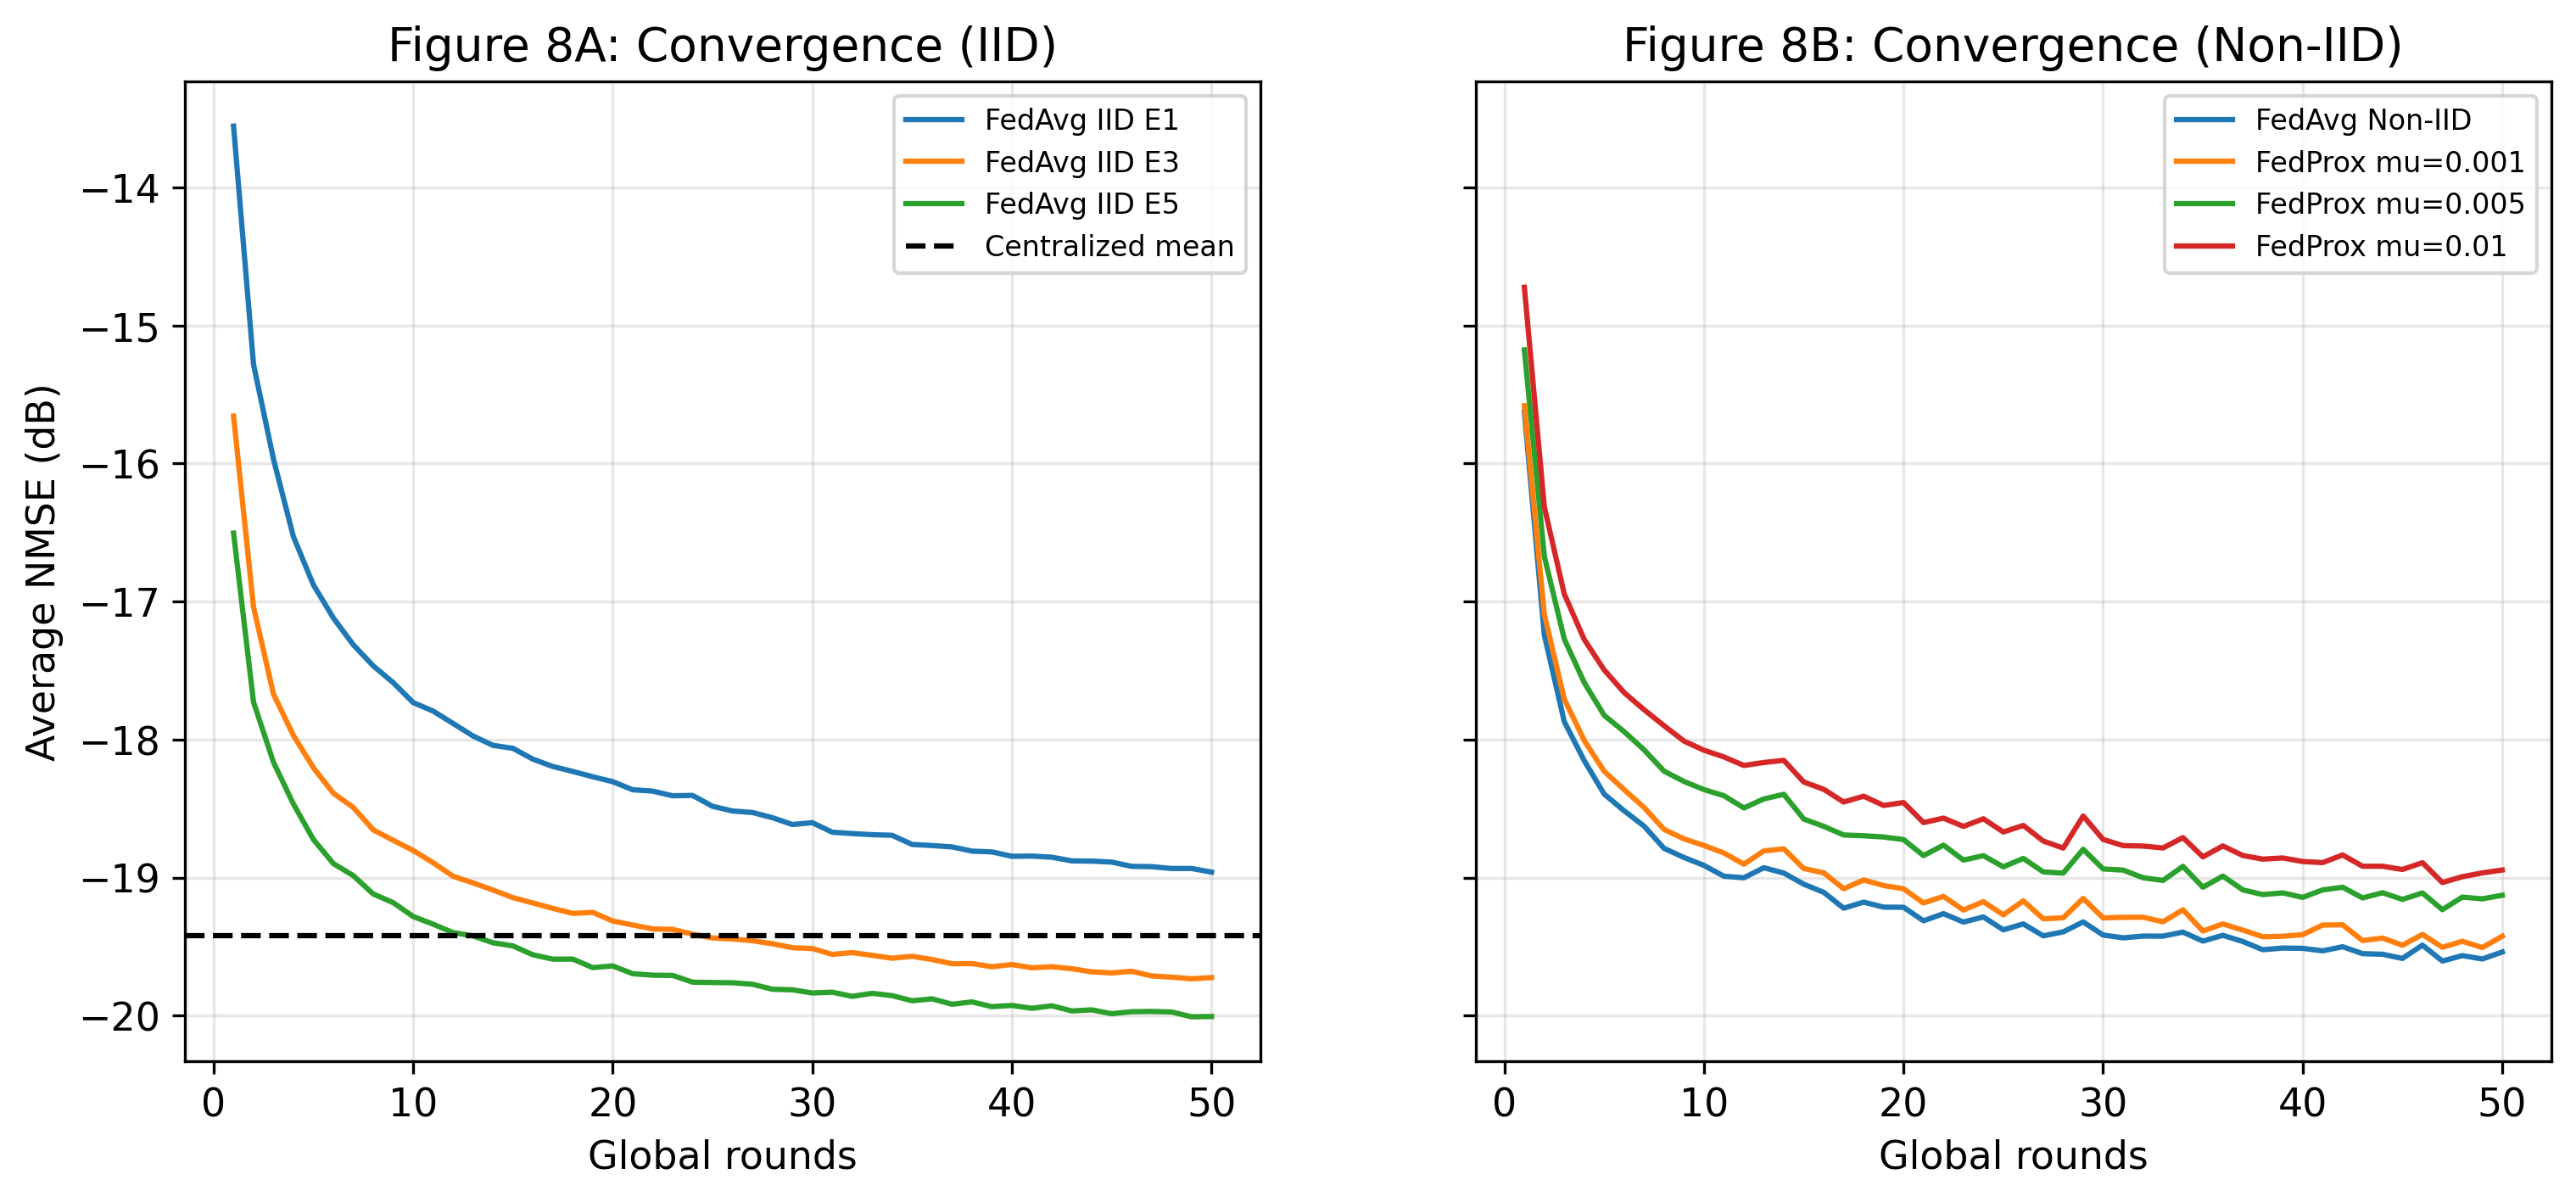
\includegraphics[width=\columnwidth]{results/figures/paper/figure8_convergence_curves.png}
\caption{Convergence trajectories for selected protocols (core figure).}
\label{fig:f8}
\end{figure}

\textbf{Observation:} IID trajectories are smoother and reach lower NMSE levels than Non-IID trajectories. Non-IID settings show slower descent and larger fluctuation, consistent with stronger objective mismatch across clients.

\textbf{Interpretation:} convergence curves confirm that heterogeneity is not only an endpoint issue; it affects optimization dynamics throughout training.

\textbf{Implication:} algorithm choice and hyperparameter tuning for Non-IID should be based on trajectory stability, not solely final NMSE.

\subsection{IID vs Non-IID and Algorithm Behavior}
\textbf{Purpose:} quantify distribution-shift penalty and analyze FedProx behavior relative to FedAvg.

\begin{figure}[t]
\centering
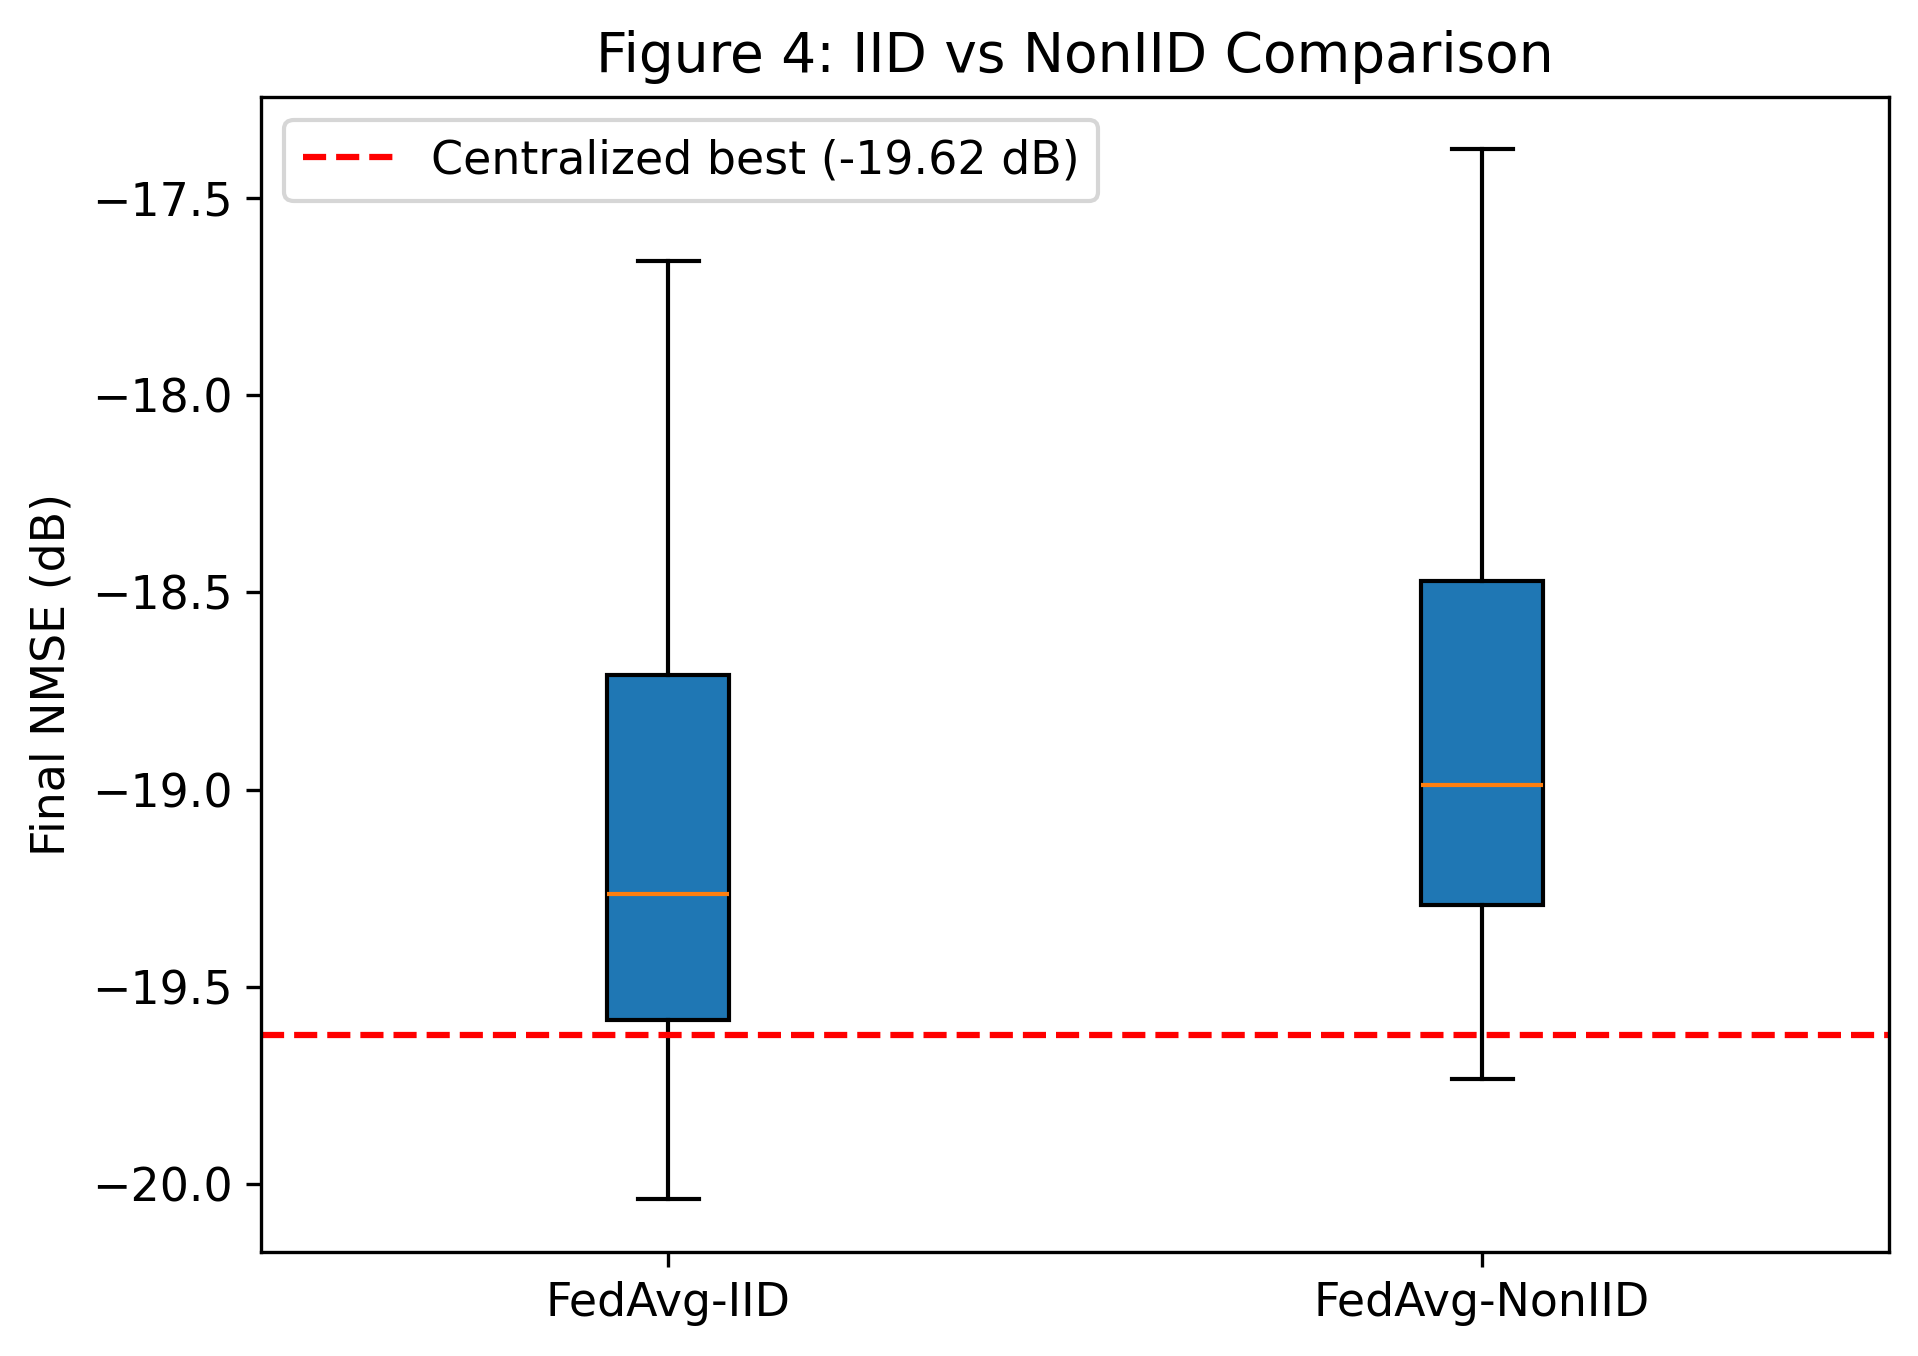
\includegraphics[width=\columnwidth]{results/figures/paper/figure4_iid_vs_noniid.png}
\caption{IID vs Non-IID distribution (purpose: direct heterogeneity penalty visualization).}
\label{fig:f4}
\end{figure}

\begin{figure}[t]
\centering
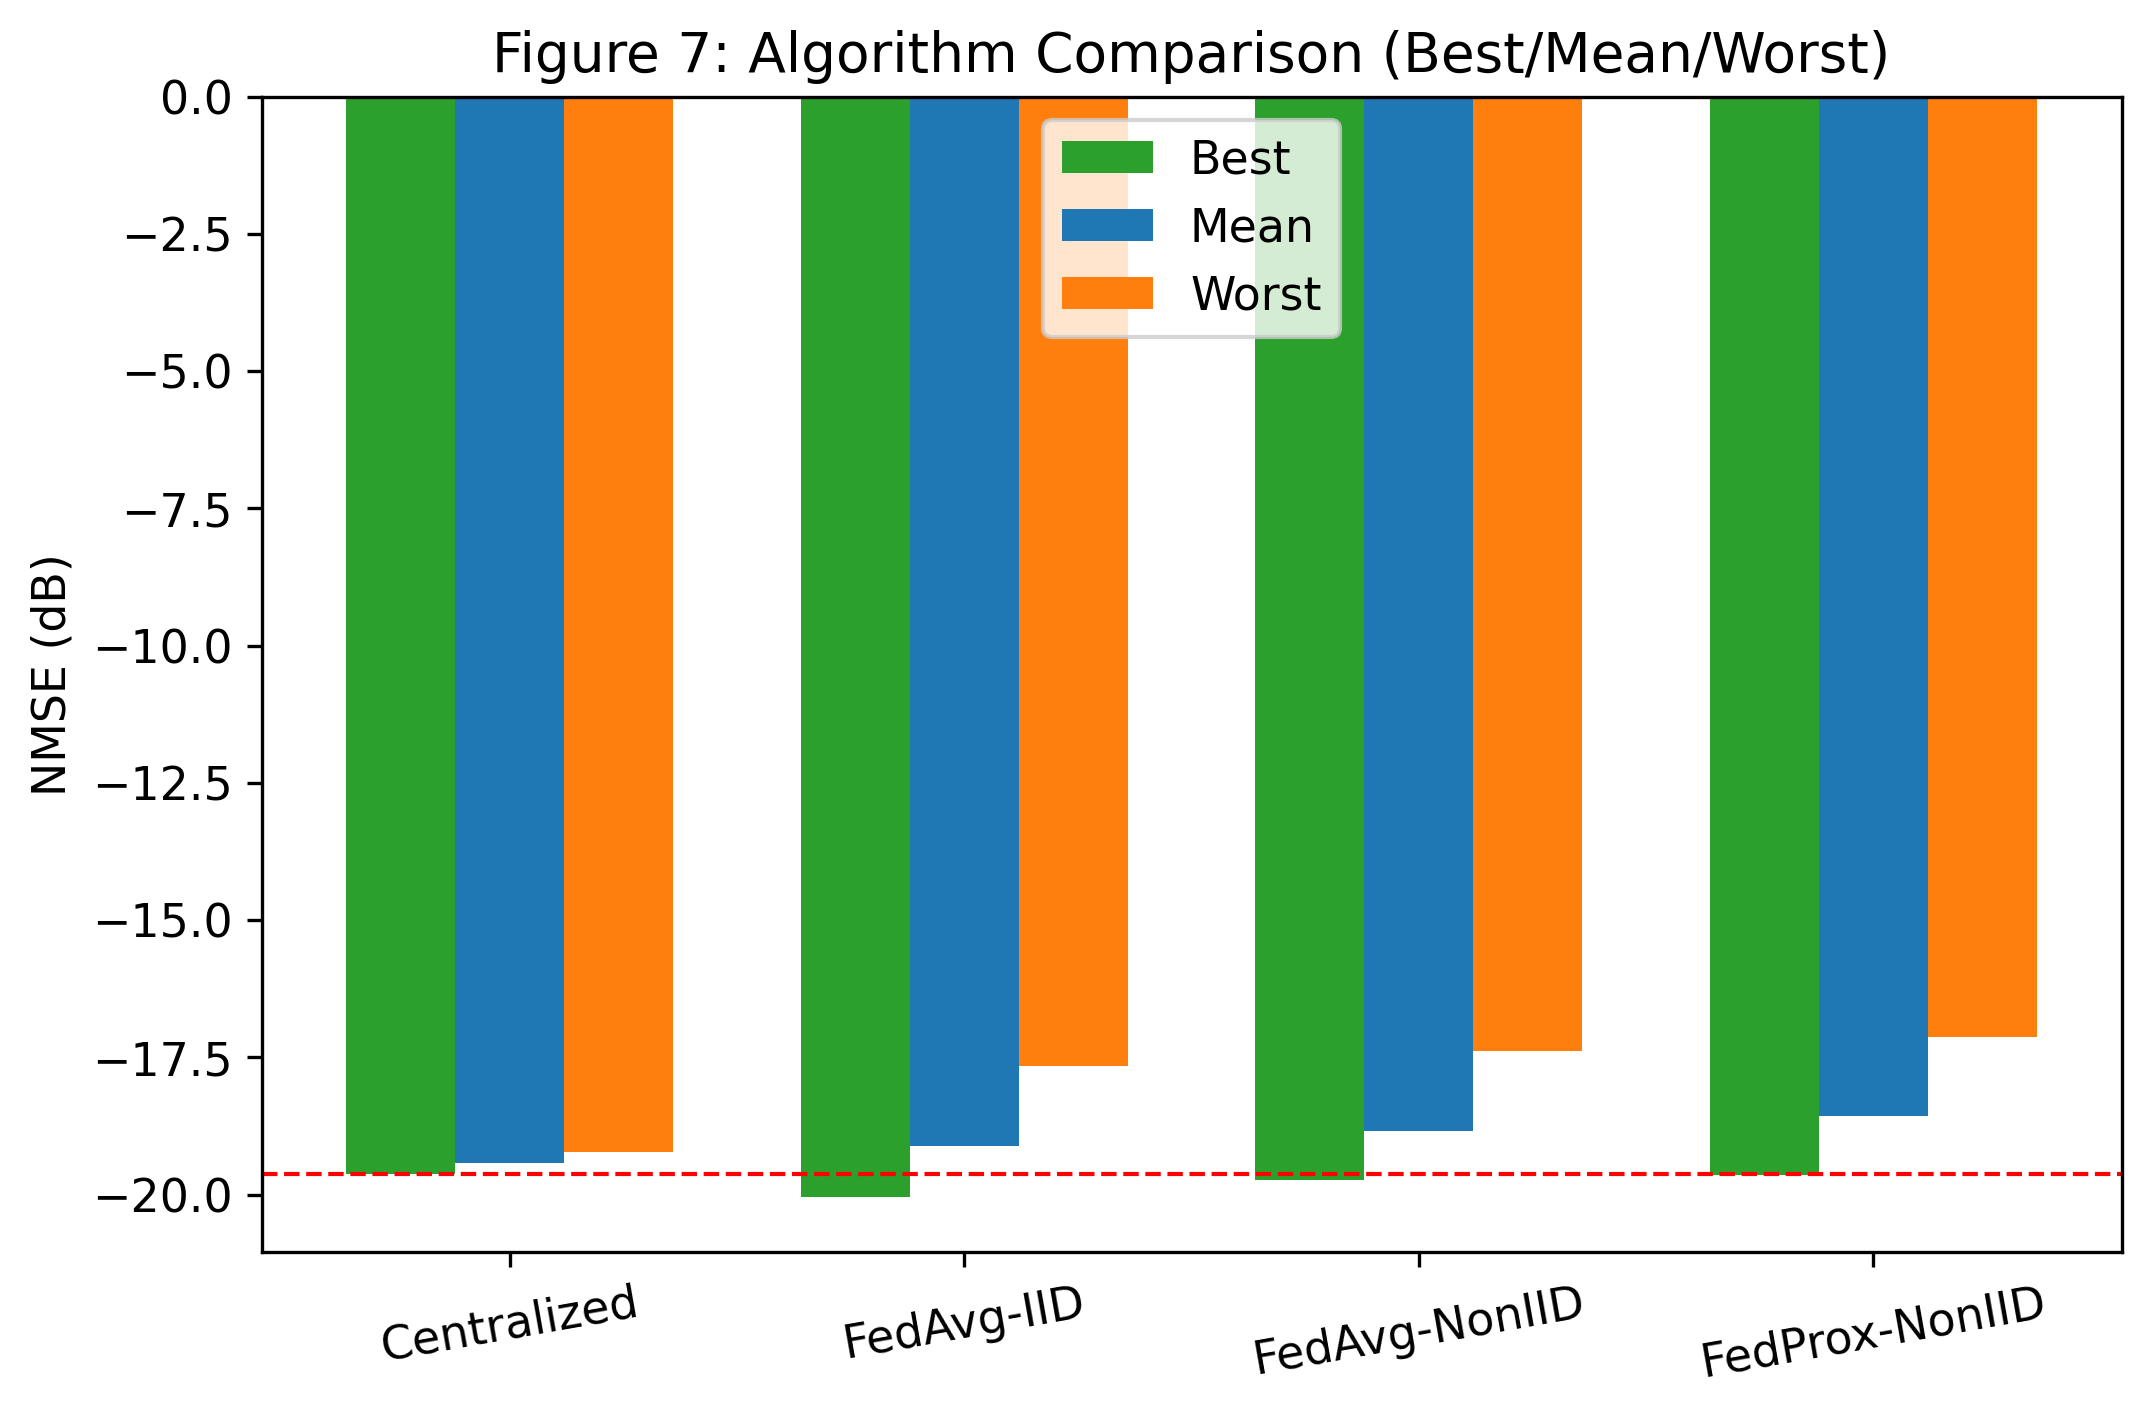
\includegraphics[width=\columnwidth]{results/figures/paper/figure7_algorithm_summary.png}
\caption{Best/mean/worst summary (purpose: variability and robustness interpretation).}
\label{fig:f7}
\end{figure}

\textbf{Observation:} Non-IID shifts distributions upward (worse NMSE). Mean gap from FedAvg-IID to FedAvg-Non-IID is +0.2707 dB. Statistical tests show this gap is significant (Welch $p=0.0289$). For FedAvg-Non-IID vs FedProx-Non-IID, the +0.2800 dB difference is also significant (Welch $p=0.0044$), favoring FedAvg on mean NMSE in this benchmark.

\textbf{Interpretation:} Non-IID impact is both measurable and statistically supported. FedProx does not uniformly improve mean NMSE; instead, its benefit appears stability-oriented and parameter-regime dependent.

\textbf{Best/mean/worst interpretation:} wider spread indicates stronger sensitivity to hyperparameters/seed; narrower spread indicates more stable behavior. Non-IID regimes show broader variability bands.

\textbf{Implication:} for production-style robustness, distribution spread and confidence bands should be reported alongside mean scores.

\subsection{Cross-Architecture Consistency (ResUNet Add-on)}
\textbf{Purpose:} test whether heterogeneity conclusions are model-specific or architecture-agnostic.

\begin{table}[t]
\caption{ResUNet Add-on Summary (5 Seeds/Setting)}
\label{tab:resunet}
\centering
\begin{tabular}{lcccc}
\toprule
Setting & Runs & Mean (dB) & Std (dB) & Best (dB) \\
\midrule
Centralized & 5 & -22.1210 & 0.3934 & -22.5281 \\
FedAvg-IID & 5 & -22.8969 & 0.1327 & -23.0406 \\
FedAvg-Non-IID & 5 & -21.1819 & 0.3369 & -21.6237 \\
FedProx-Non-IID & 5 & -20.4661 & 0.1393 & -20.6357 \\
\bottomrule
\end{tabular}
\end{table}

\begin{figure}[t]
\centering
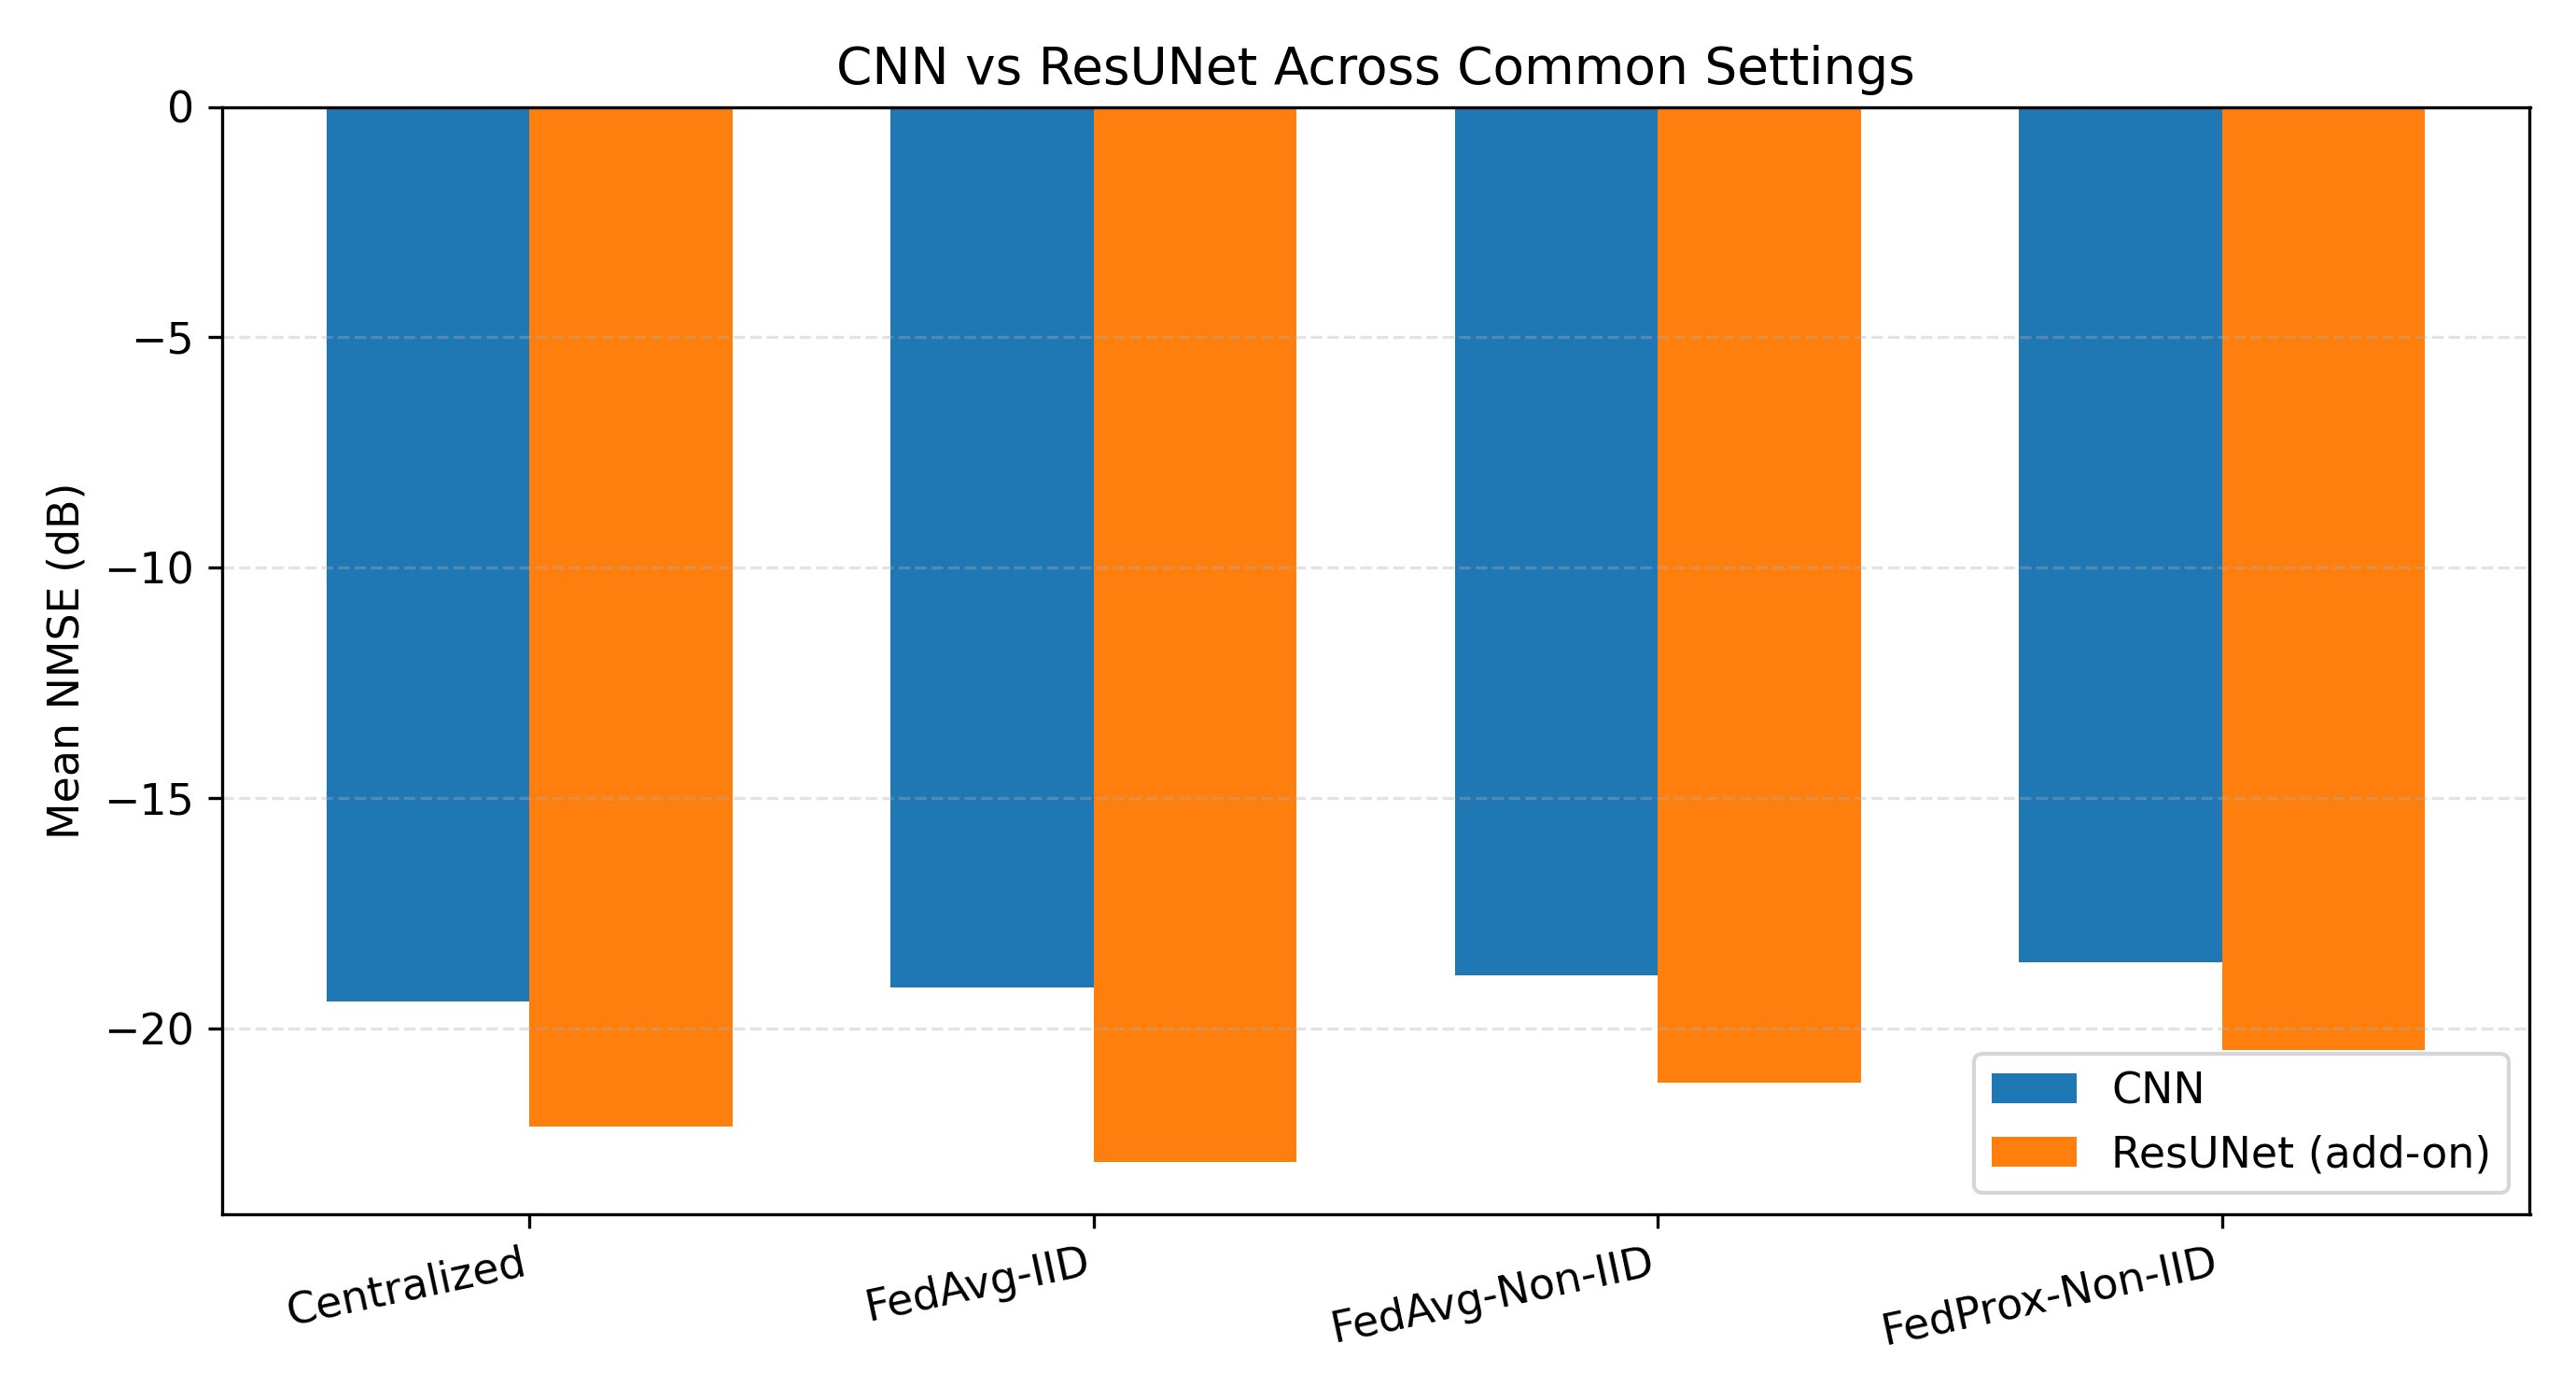
\includegraphics[width=\columnwidth]{results/figures/paper/resunet_addon_cnn_vs_resunet.png}
\caption{CNN vs ResUNet under aligned settings (purpose: trend portability across architectures).}
\label{fig:cross}
\end{figure}

\textbf{Observation:} ResUNet reproduces core trend directions: FedAvg-IID is strongest federated setting, and Non-IID causes substantial degradation. Specifically, FedAvg-Non-IID degrades by +1.7150 dB vs FedAvg-IID.

\textbf{Interpretation:} heterogeneity penalty persists across shallow and encoder-decoder architectures, indicating a data-distribution effect rather than a single-model artifact.

\textbf{Implication:} mitigation strategies for Non-IID should be treated as pipeline-level priorities, not architecture-only fixes.

\subsection{Classical Baseline and Communication Analysis}
\textbf{Purpose:} place deep models relative to classical LS and quantify systems cost.

\begin{table}[t]
\caption{Classical and Deep Baselines at 10 dB}
\label{tab:ls}
\centering
\begin{tabular}{lcc}
\toprule
Method & NMSE (dB) & Note \\
\midrule
LS & -9.9631 & $\hat H=H_{noisy}$ \\
CNN (CL mean) & -19.4227 & +9.46 dB vs LS \\
ResUNet (CL mean) & -22.1210 & +12.16 dB vs LS \\
\bottomrule
\end{tabular}
\end{table}

\textbf{Observation:} deep models significantly outperform LS at 10 dB. CNN and ResUNet centralized means improve over LS by +9.46 dB and +12.16 dB, respectively.

Communication payload model (FP32):
\begin{equation}
\mathcal{C}_{\text{round}}\approx 4P,\qquad
\mathcal{C}_{\text{total}}\approx 4PKR.
\end{equation}
For $K{=}5, R{=}50$: CNN (19,778 params) requires \~18.86 MB total uplink payload, while ResUNet (763,234 params) requires \~727.88 MB.

\textbf{Interpretation:} communication burden scales linearly with both model size and federated rounds. The architecture that improves NMSE the most may also be the least communication-efficient.

\textbf{Implication:} communication-aware model selection is essential for realistic FL deployment; NMSE alone is insufficient.

\begin{table}[t]
\caption{Communication Cost Snapshot (CNN)}
\label{tab:comm}
\centering
\begin{tabular}{lccc}
\toprule
Configuration & Comm. Events & NMSE (dB) & Efficiency \\
\midrule
FedAvg-IID (R10,E1) & 50 & -17.7319 & Low \\
FedAvg-IID (R30,E3) & 150 & -19.5375 & Medium \\
FedAvg-IID (R50,E5) & 250 & -20.0190 & High \\
Centralized (20 ep) & 0 & -19.4227 & -- \\
\bottomrule
\end{tabular}
\end{table}

\section{Comparison With Prior Published Work}
The closest domain reference is Elbir and Coleri~\cite{elbir2021flchannel}. We align on FL-based channel estimation objective and communication-overhead motivation. Exact protocol assumptions differ (scenario specifics, model details, split policies), so comparison is presented as partially matched rather than direct leaderboard equivalence.

\subsection{What We Adopt From Elbir--Coleri}
Their paper establishes a clear systems-oriented framing: CL requires transmission of user datasets to the BS, whereas FL transmits model updates only, reducing communication burden while maintaining estimation performance close to CL~\cite{elbir2021flchannel}. We adopt this framing in our manuscript structure and report pipeline-level trade-offs rather than only endpoint NMSE values.

Concretely, their methodology includes: (i) FL channel estimation in both conventional and RIS-assisted massive MIMO, (ii) communication-overhead analysis versus CL, and (iii) robustness checks under noisy/quantized/lossy model-update transmission. Their reported headline includes approximately 16$\times$ lower communication overhead versus CL in their setup.

\subsection{Detailed Alignment and Differences}
To make comparison effective and reviewer-safe, Table~\ref{tab:alignment_ec} itemizes what is directly aligned and what is only contextually comparable.

\begin{table}[t]
\caption{Detailed Alignment With Elbir--Coleri~\cite{elbir2021flchannel}}
\label{tab:alignment_ec}
\centering
\begin{tabular}{p{0.25\linewidth}p{0.34\linewidth}p{0.30\linewidth}}
\toprule
Aspect & Elbir--Coleri (TWC) & This Work \\
\midrule
Primary motivation & Reduce CL data-transfer overhead via FL & Same motivation and FL framing \\
Task & FL channel estimation & FL channel estimation \\
Scenarios & Conventional + RIS-assisted massive MIMO & Massive MIMO benchmark (DeepMIMO O1\_60) \\
Model family & CNN-based ChannelNet & CNN (primary) + ResUNet (add-on) \\
Learning modes & CL vs FL & CL vs FL (FedAvg/FedProx) \\
Heterogeneity analysis & Non-i.i.d. challenge discussed & Explicit IID/Non-IID protocol and quantified deltas \\
Update-channel robustness & Noisy, quantized, partial-loss model updates & Communication/runtime analysis; update-channel robustness left for future extension \\
Overhead reporting & Reports \textasciitilde16$\times$ lower overhead vs CL & Communication events + payload model (4PKR) \\
Comparison level & Domain reference benchmark & Partial-match external comparison \\
\bottomrule
\end{tabular}
\end{table}

\subsection{Effective Comparison Statement}
Our results should be interpreted as \emph{consistent with} the Elbir--Coleri systems conclusion, not as a strict protocol-identical replacement. Specifically, both studies support the practical value of FL for channel estimation under communication constraints; our work additionally emphasizes reproducibility, IID/Non-IID quantification, and cross-architecture trend validation. At the same time, we explicitly separate direct comparisons from partially matched ones due to differences in scenario construction (e.g., RIS-inclusive setup, robustness tests on update transmission, and model-design choices).

\begin{table}[t]
\caption{Comparison Framing With Prior Work}
\label{tab:prior}
\centering
\begin{tabular}{p{0.28\linewidth}p{0.29\linewidth}p{0.31\linewidth}}
\toprule
Dimension & This Work & Elbir--Coleri~\cite{elbir2021flchannel} \\
\midrule
Task & FL channel estimation & FL channel estimation \\
Core algorithms & FedAvg/FedProx & FL-CNN framework \\
Main metric & NMSE (dB) & Estimation error/NMSE style \\
Overhead framing & Explicit comm events + payload model & Reports major overhead reduction vs CL \\
Comparability & Partial-match & Partial-match \\
\bottomrule
\end{tabular}
\end{table}

\section{Discussion}
\subsection{Why ResUNet tends to perform better}
ResUNet combines multiscale encoder-decoder representation and skip-connections, which preserve structural detail while denoising. This appears beneficial for complex channel reconstruction beyond shallow CNN capacity.

\subsection{Why Non-IID hurts}
Non-IID clients optimize diverging local objectives; aggregation then combines updates with larger directional disagreement, reducing final global fit quality and increasing sensitivity.

\subsection{Why FedProx can be inconsistent}
FedProx regularization ($\mu$) can stabilize updates but also restrict local adaptation. Benefit depends on heterogeneity level, local epochs, and model capacity; therefore, stability and accuracy may not improve simultaneously.

\section{Limitations and Future Work}
\subsection{Limitations}
\begin{itemize}
    \item Current full federated matrix is centered at 10 dB.
    \item MMSE is not integrated with matched covariance calibration in this release.
    \item ResUNet is an add-on validation (not full-grid sweep).
    \item External comparison is partially matched due to protocol differences.
\end{itemize}

\subsection{Future Work}
\begin{itemize}
    \item Complete full multi-SNR federated sweeps (0/5/10/15/20 dB) for robustness profiling.
    \item Add calibrated MMSE baseline with pilot-aware covariance estimation.
    \item Extend to additional DeepMIMO scenarios for cross-environment generalization.
    \item Evaluate personalization and client-adaptive FL variants for strong Non-IID settings.
    \item Add architecture-component ablation (skip/residual depth/channel width) under matched communication budgets.
\end{itemize}

\section{Conclusion}
We presented a reproducible FL benchmark for massive MIMO channel estimation under IID and Non-IID client data, with CNN as the primary benchmark and ResUNet as add-on validation. Detailed result analysis shows three stable findings: (i) FL can achieve competitive channel estimation quality relative to centralized baselines, (ii) Non-IID client distributions introduce a consistent and statistically supported performance penalty, and (iii) communication and model size materially affect deployability, requiring joint accuracy-efficiency optimization. By coupling structured run logging, statistical summaries, core convergence evidence, and supplementary diagnostics, the study provides a transparent IEEE-style evaluation template for future FL channel-estimation research.

\section*{Supplementary Figures and Explanations}
The following figures are retained as supplementary evidence and can be moved between main text and appendix based on page budget.

\begin{figure}[t]
\centering
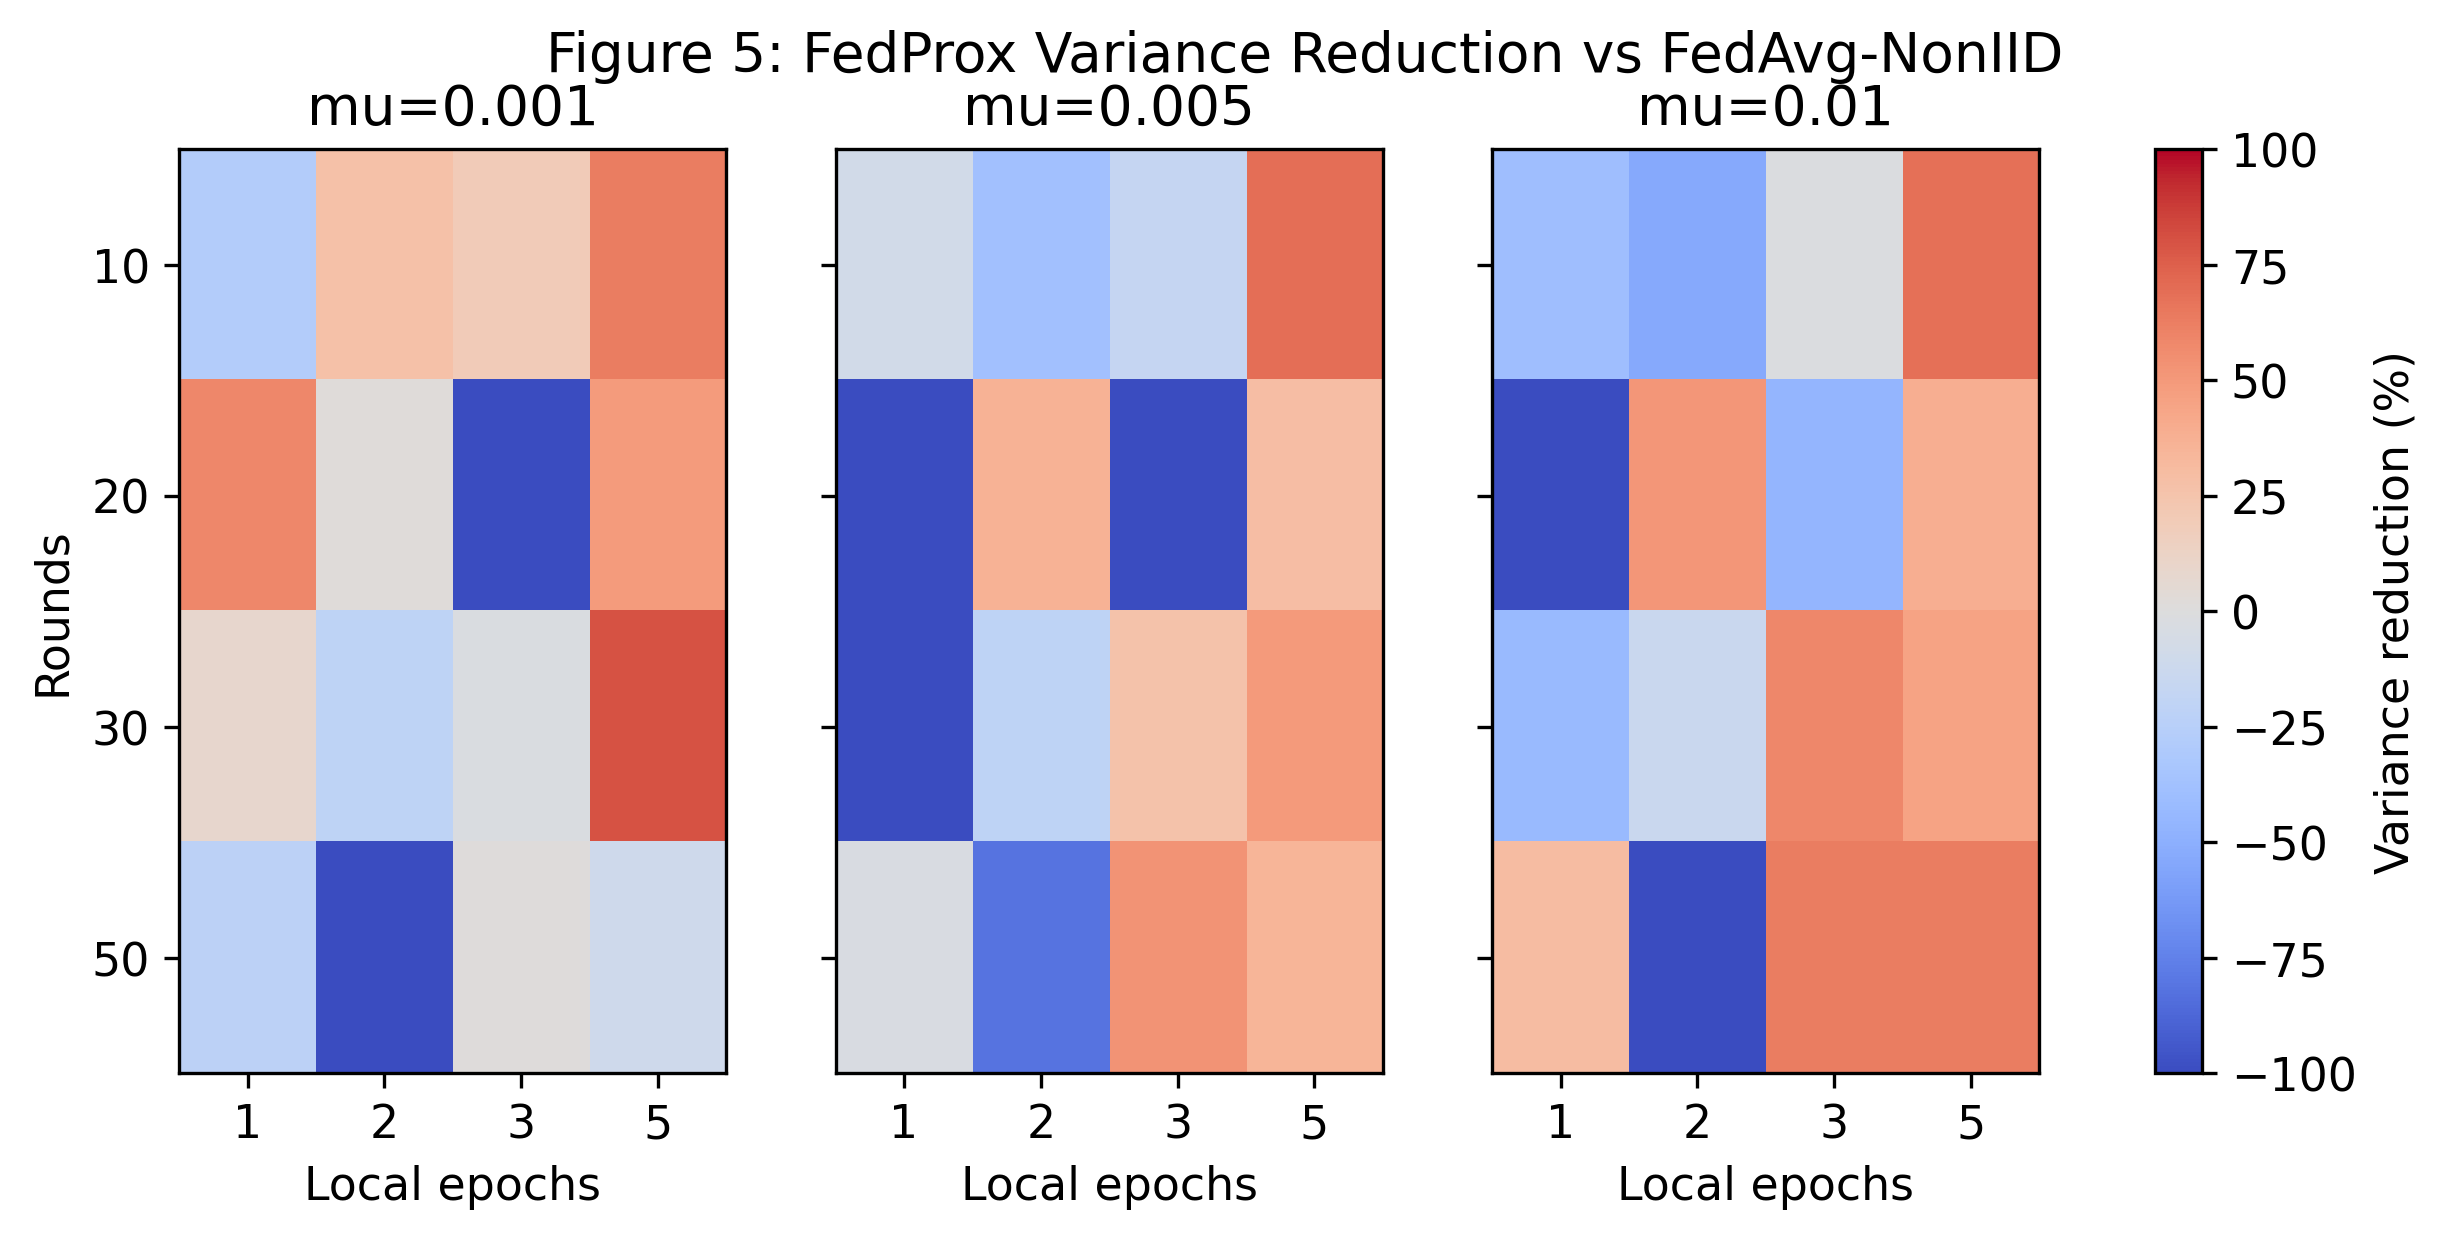
\includegraphics[width=\columnwidth]{results/figures/paper/figure5_fedprox_variance_reduction.png}
\caption{Supplementary S1: FedProx variance map. Shows where variance reduction appears even without mean accuracy gains.}
\label{fig:s1}
\end{figure}

\begin{figure}[t]
\centering
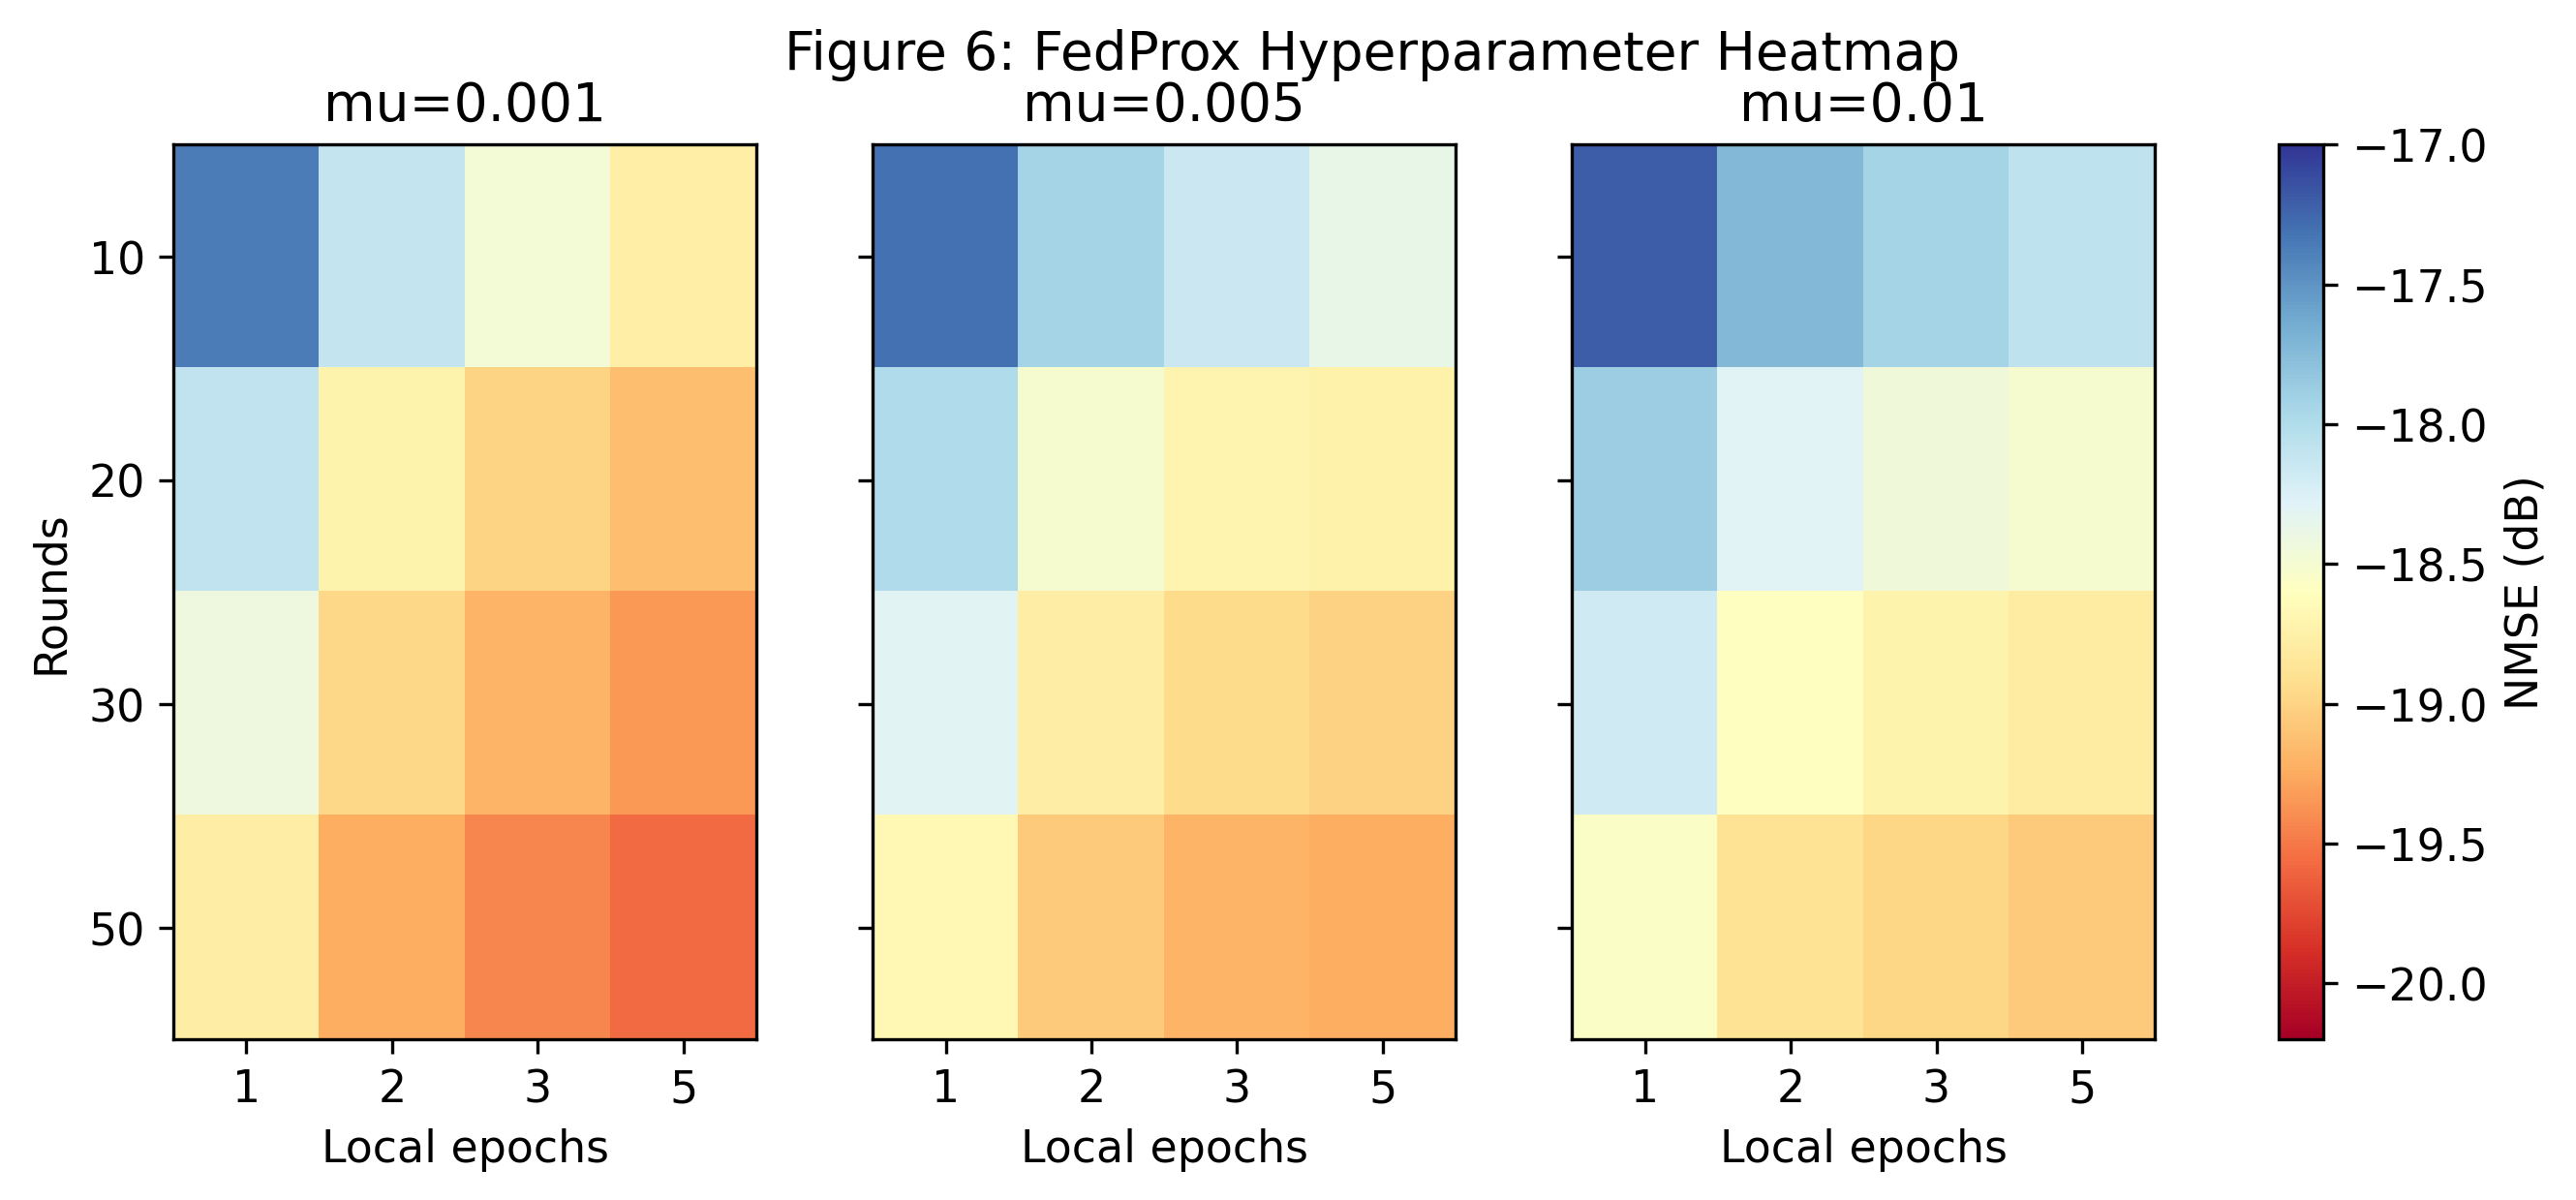
\includegraphics[width=\columnwidth]{results/figures/paper/figure6_fedprox_heatmap.png}
\caption{Supplementary S2: FedProx hyperparameter heatmap ($\mu$, rounds, epochs). Highlights sensitivity region and best-performing area.}
\label{fig:s2}
\end{figure}

\begin{figure}[t]
\centering
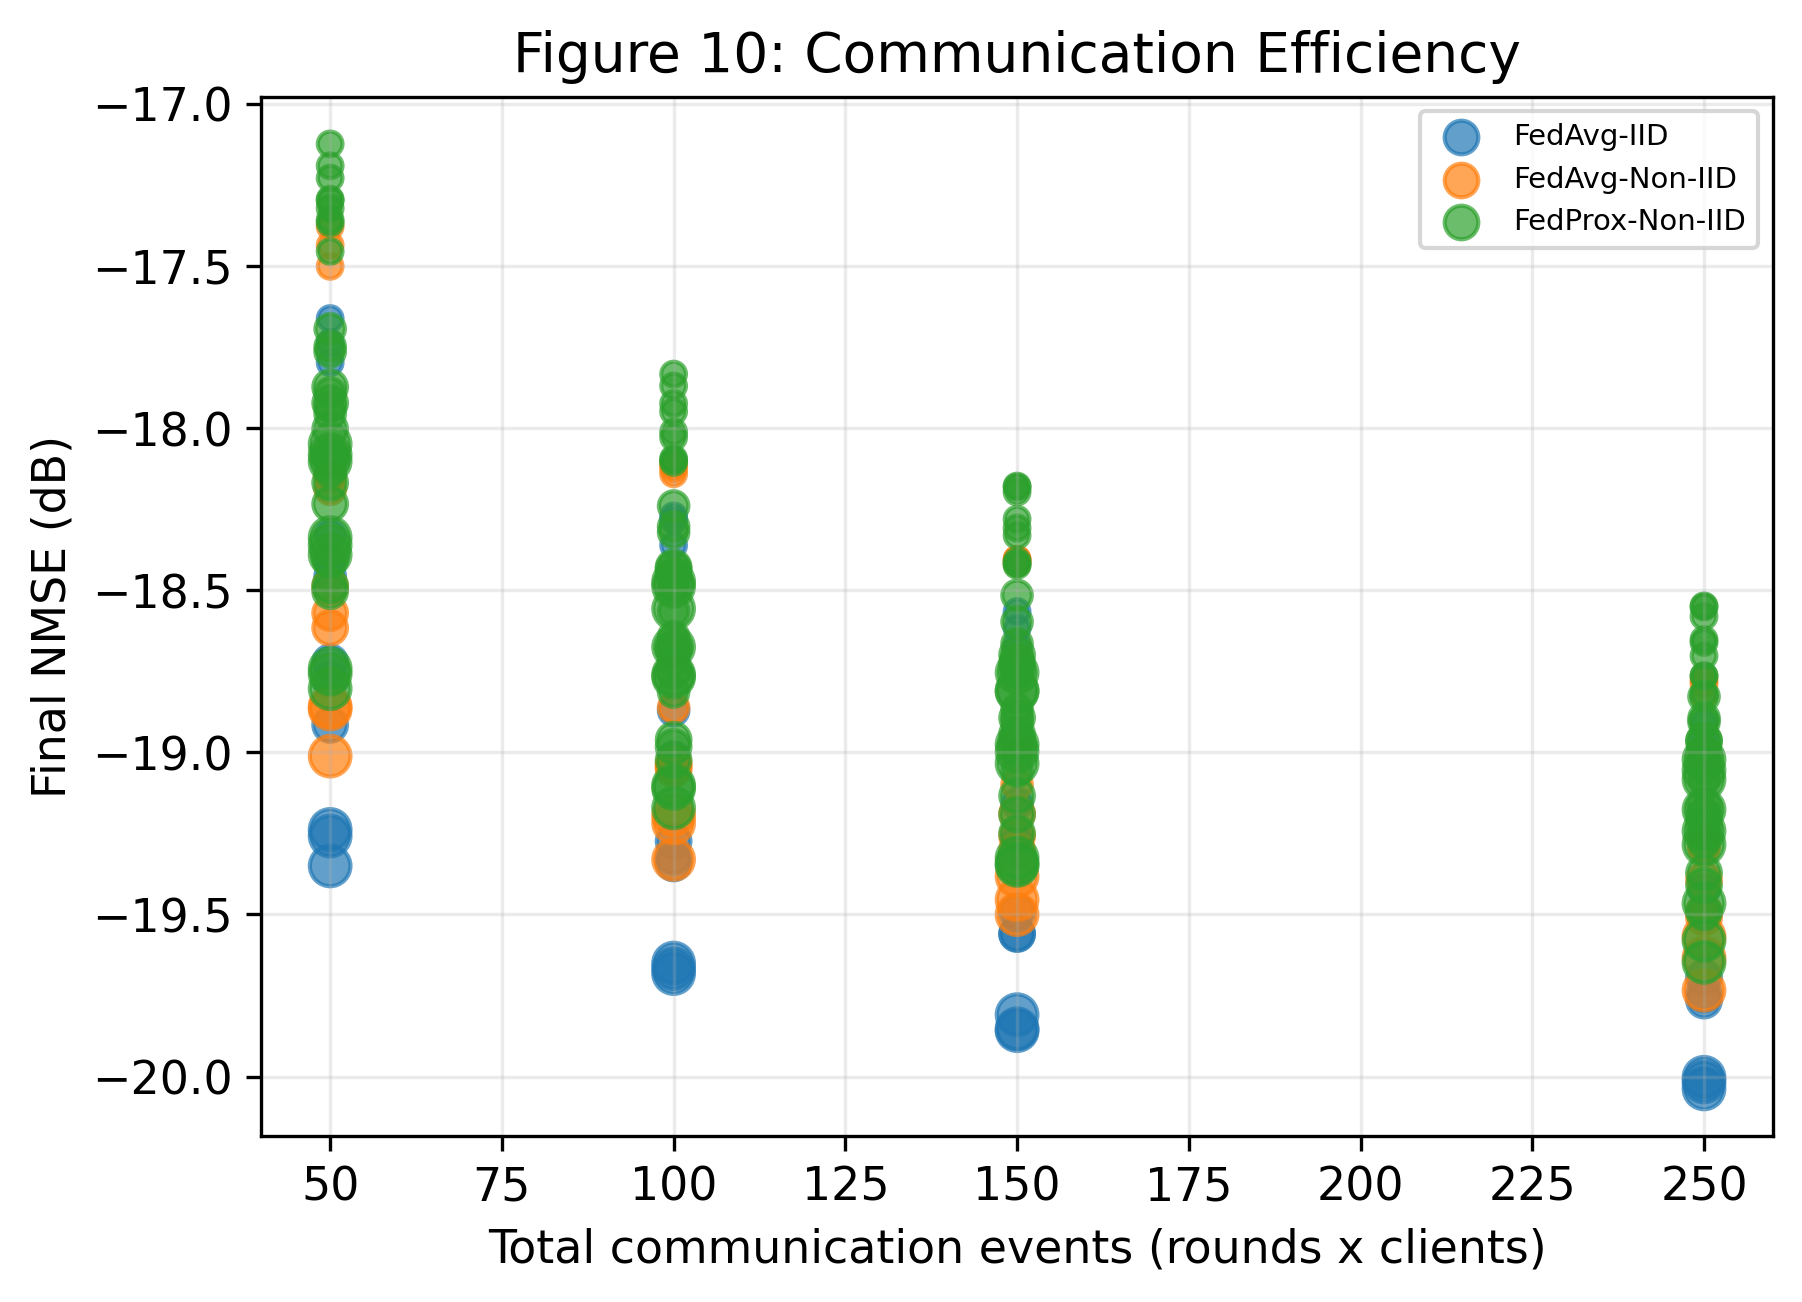
\includegraphics[width=\columnwidth]{results/figures/paper/figure10_communication_efficiency.png}
\caption{Supplementary S4: Communication-efficiency scatter. Visualizes Pareto behavior between communication events and NMSE.}
\label{fig:s4}
\end{figure}

\begin{figure}[t]
\centering
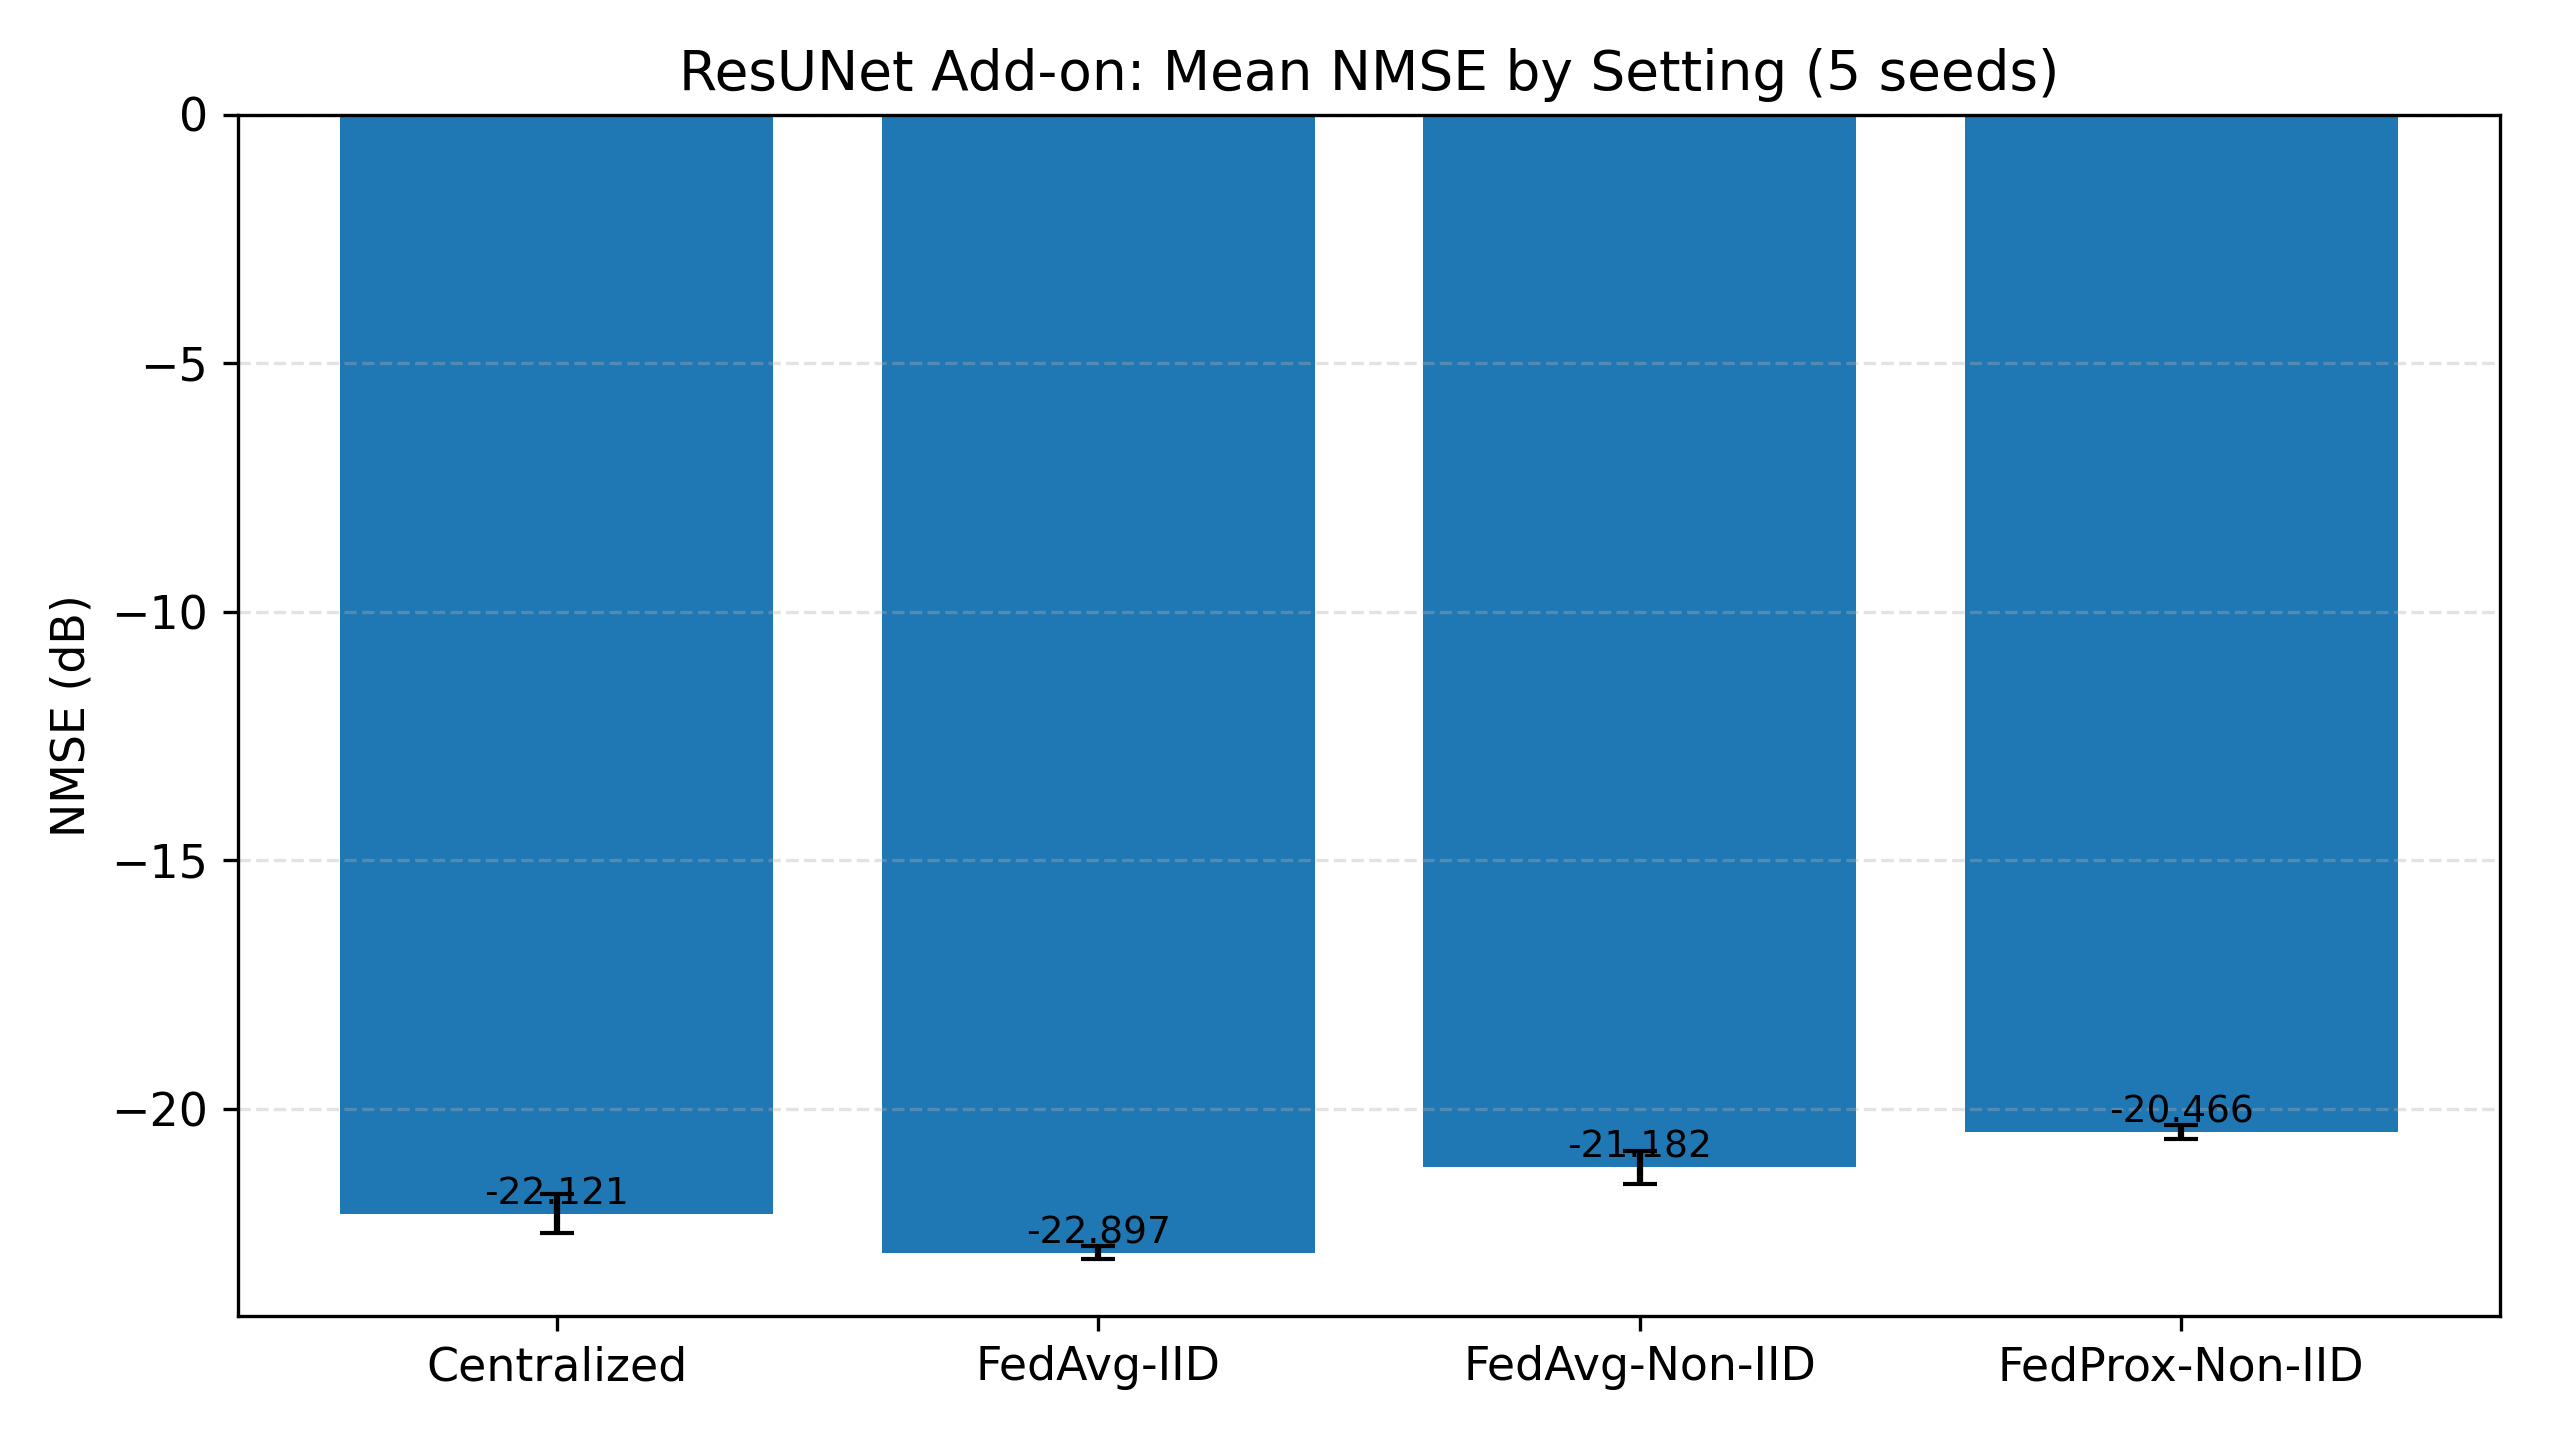
\includegraphics[width=\columnwidth]{results/figures/paper/resunet_addon_nmse_bar.png}
\caption{Supplementary S5: ResUNet add-on mean with error bars. Confirms trend consistency under architecture change.}
\label{fig:s5}
\end{figure}

\begin{figure}[t]
\centering
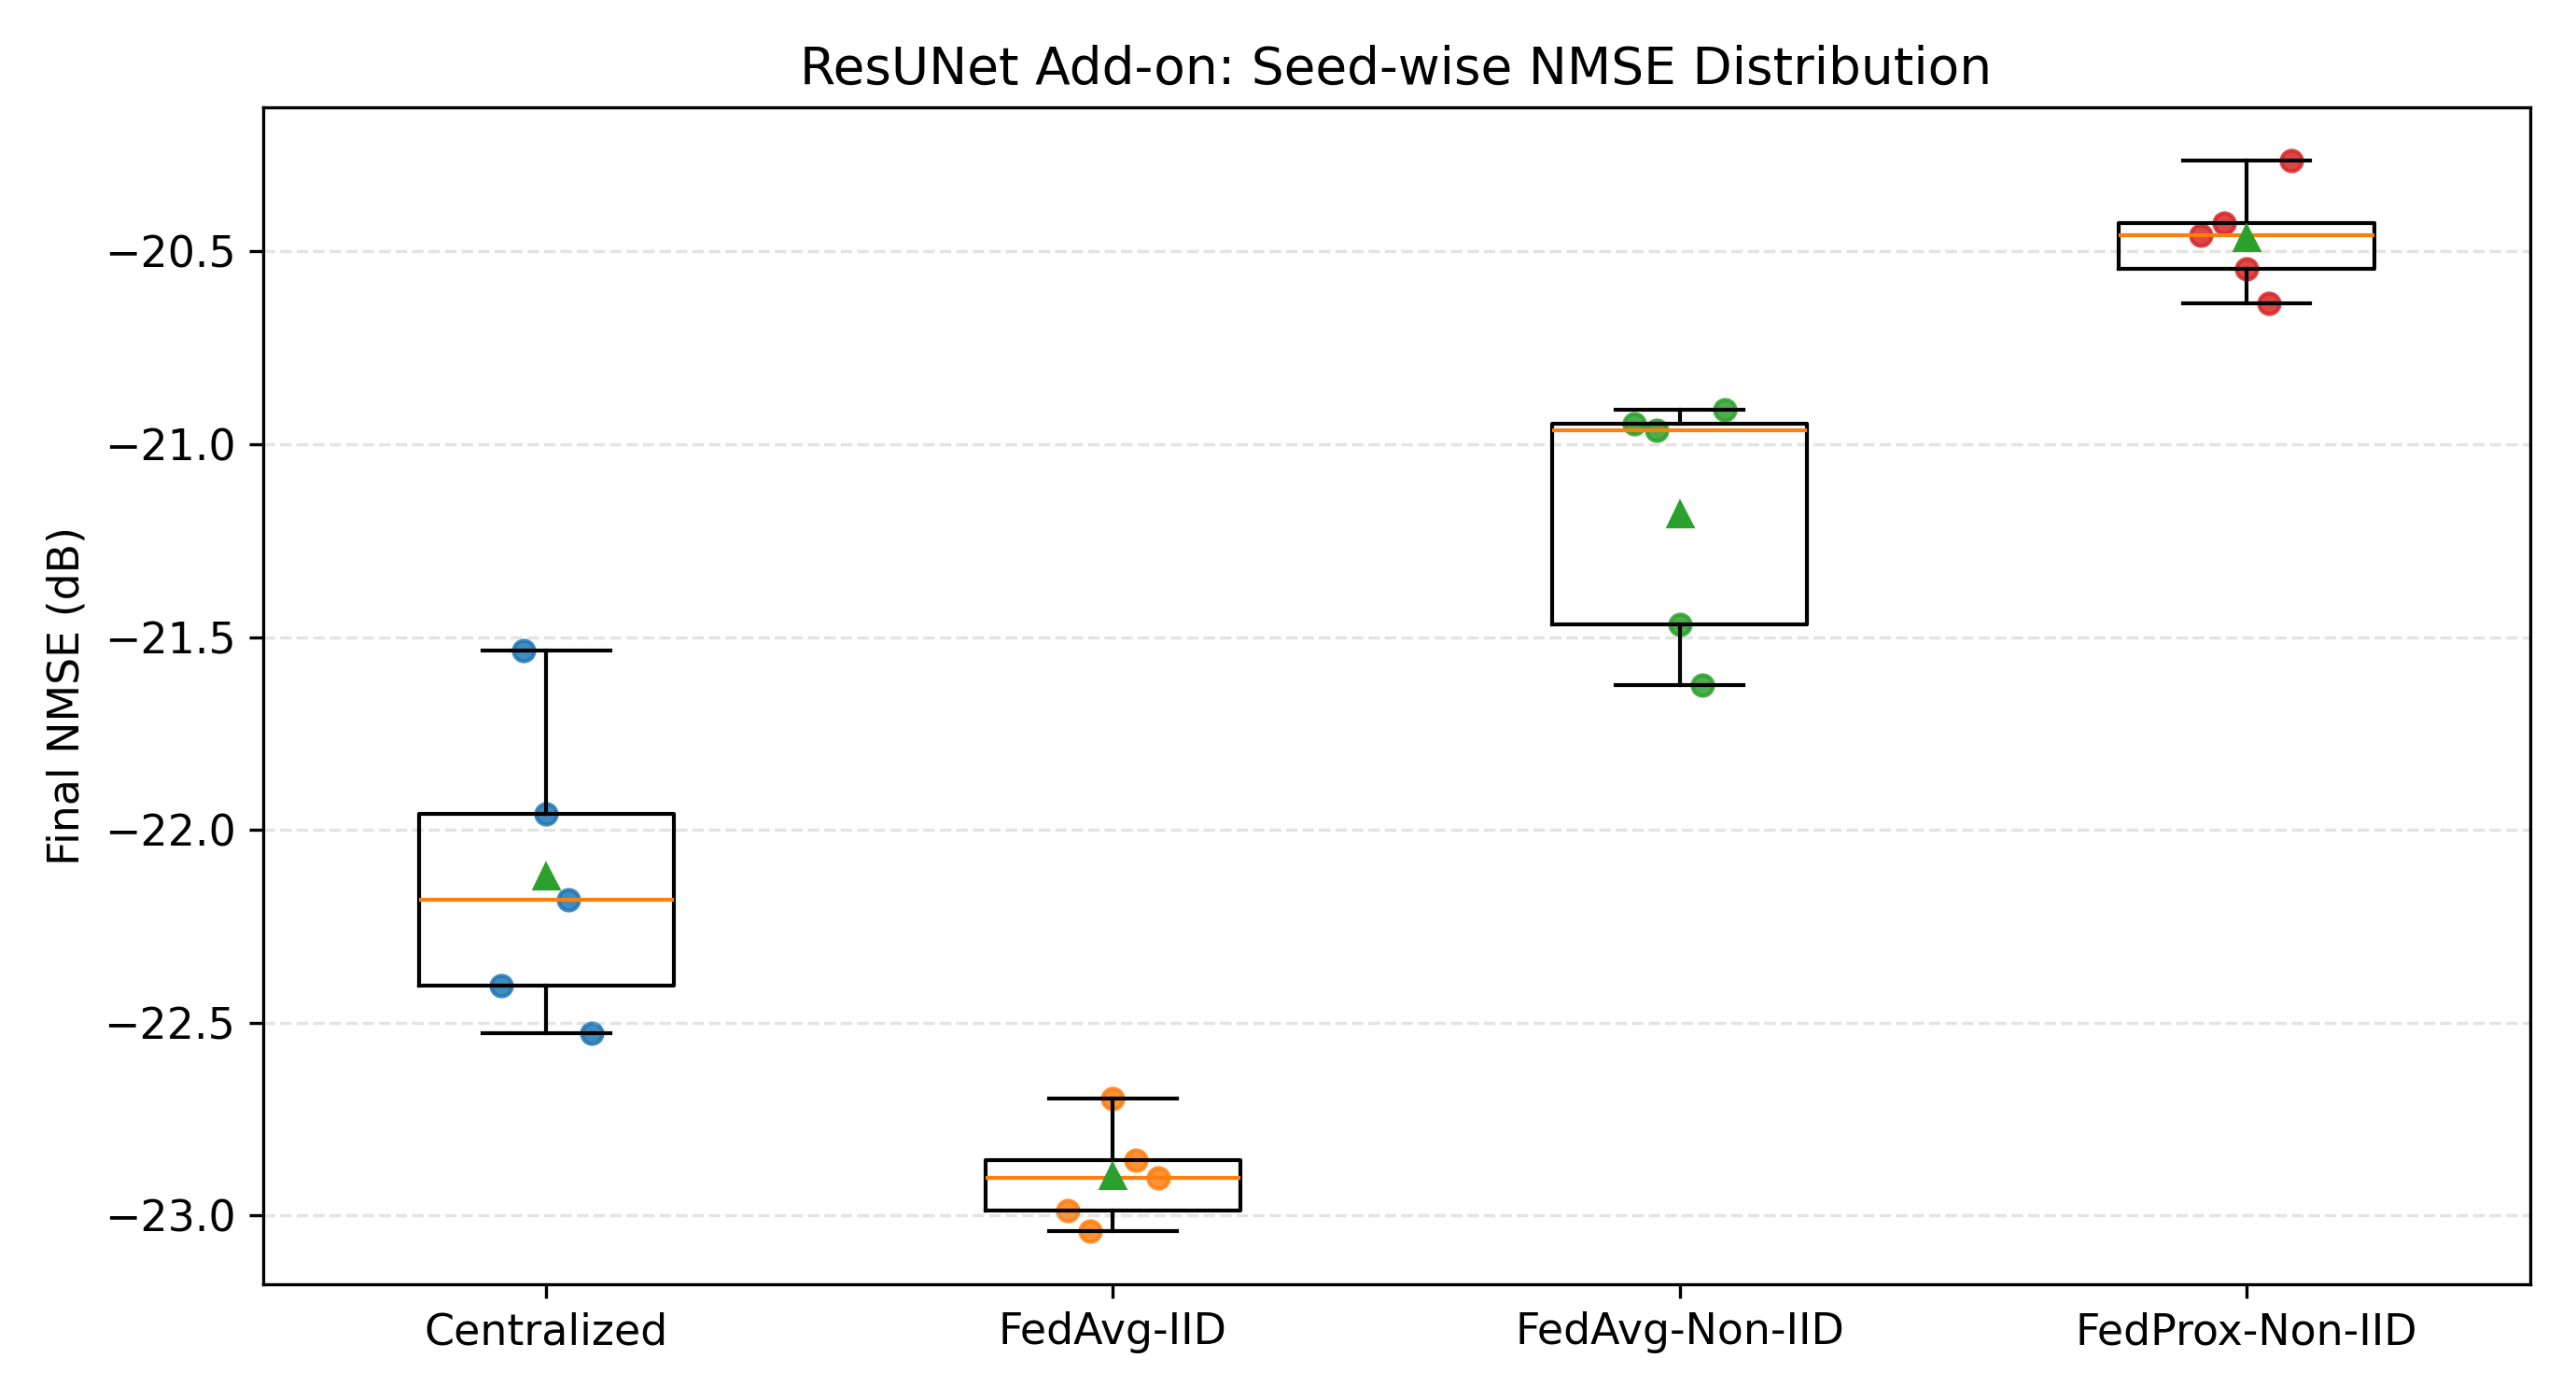
\includegraphics[width=\columnwidth]{results/figures/paper/resunet_addon_nmse_box.png}
\caption{Supplementary S6: ResUNet seed-wise distribution. Provides transparent variability view per setting.}
\label{fig:s6}
\end{figure}

\begin{figure}[t]
\centering
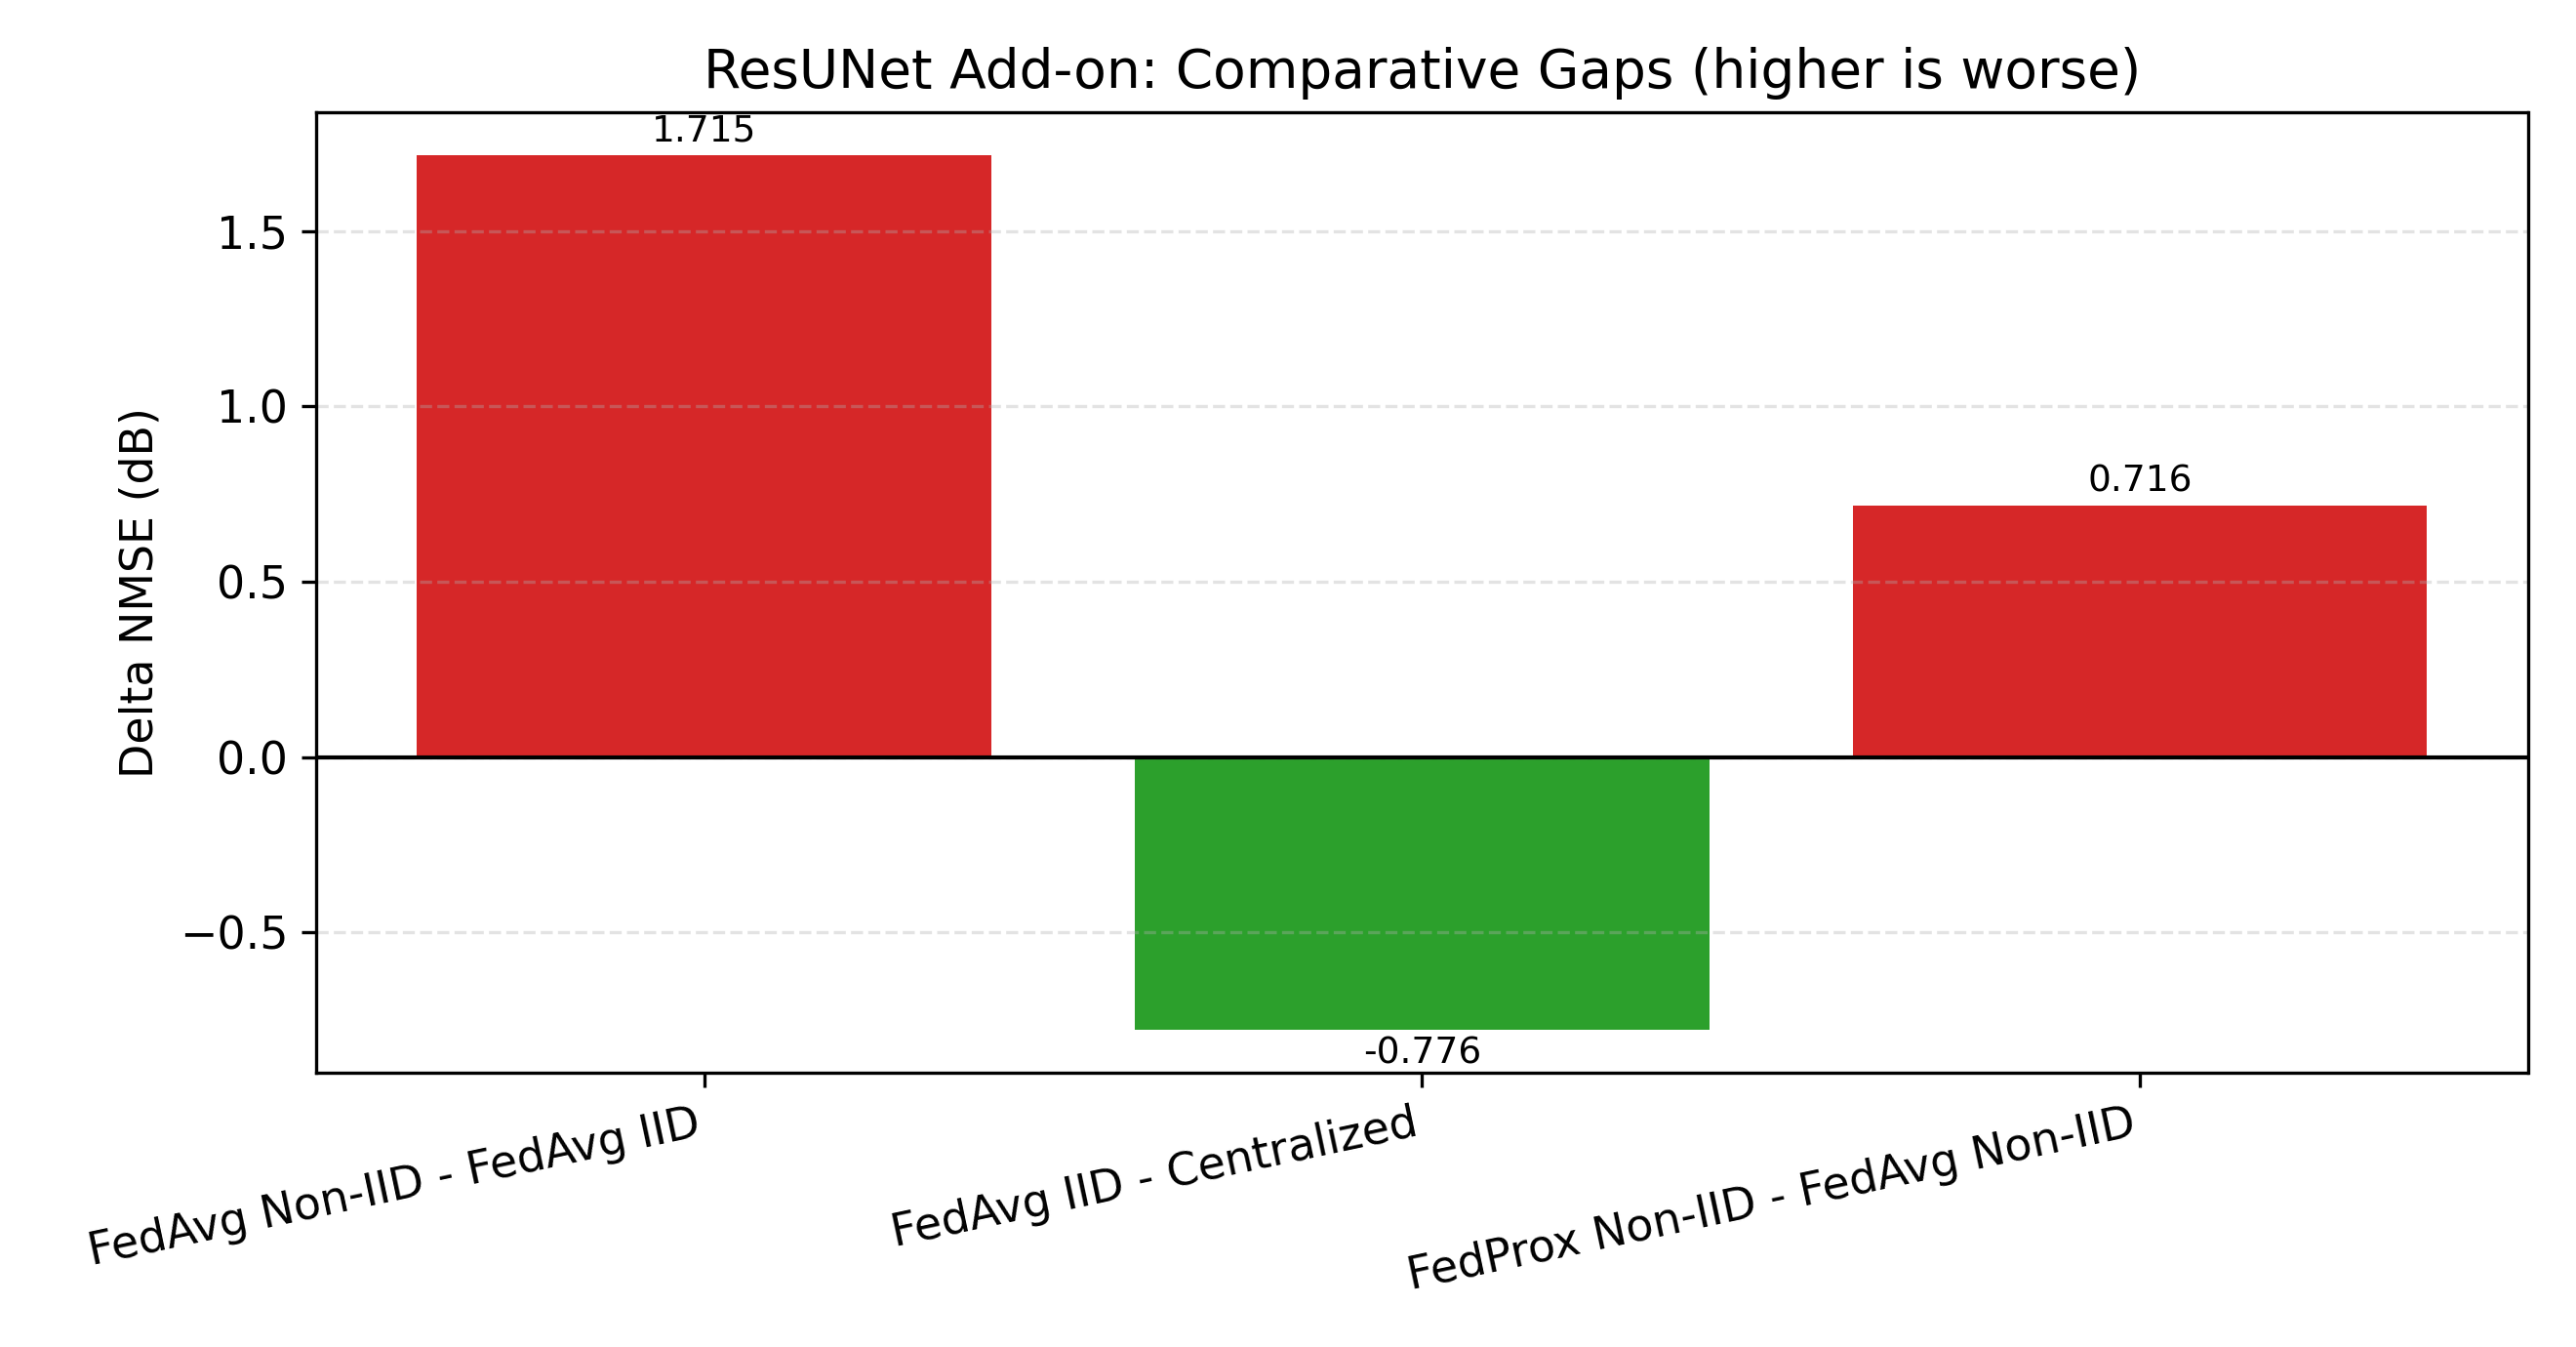
\includegraphics[width=\columnwidth]{results/figures/paper/resunet_addon_gap_analysis.png}
\caption{Supplementary S7: ResUNet delta analysis (IID/Non-IID/FedProx effects).}
\label{fig:s7}
\end{figure}

\begin{figure}[t]
\centering
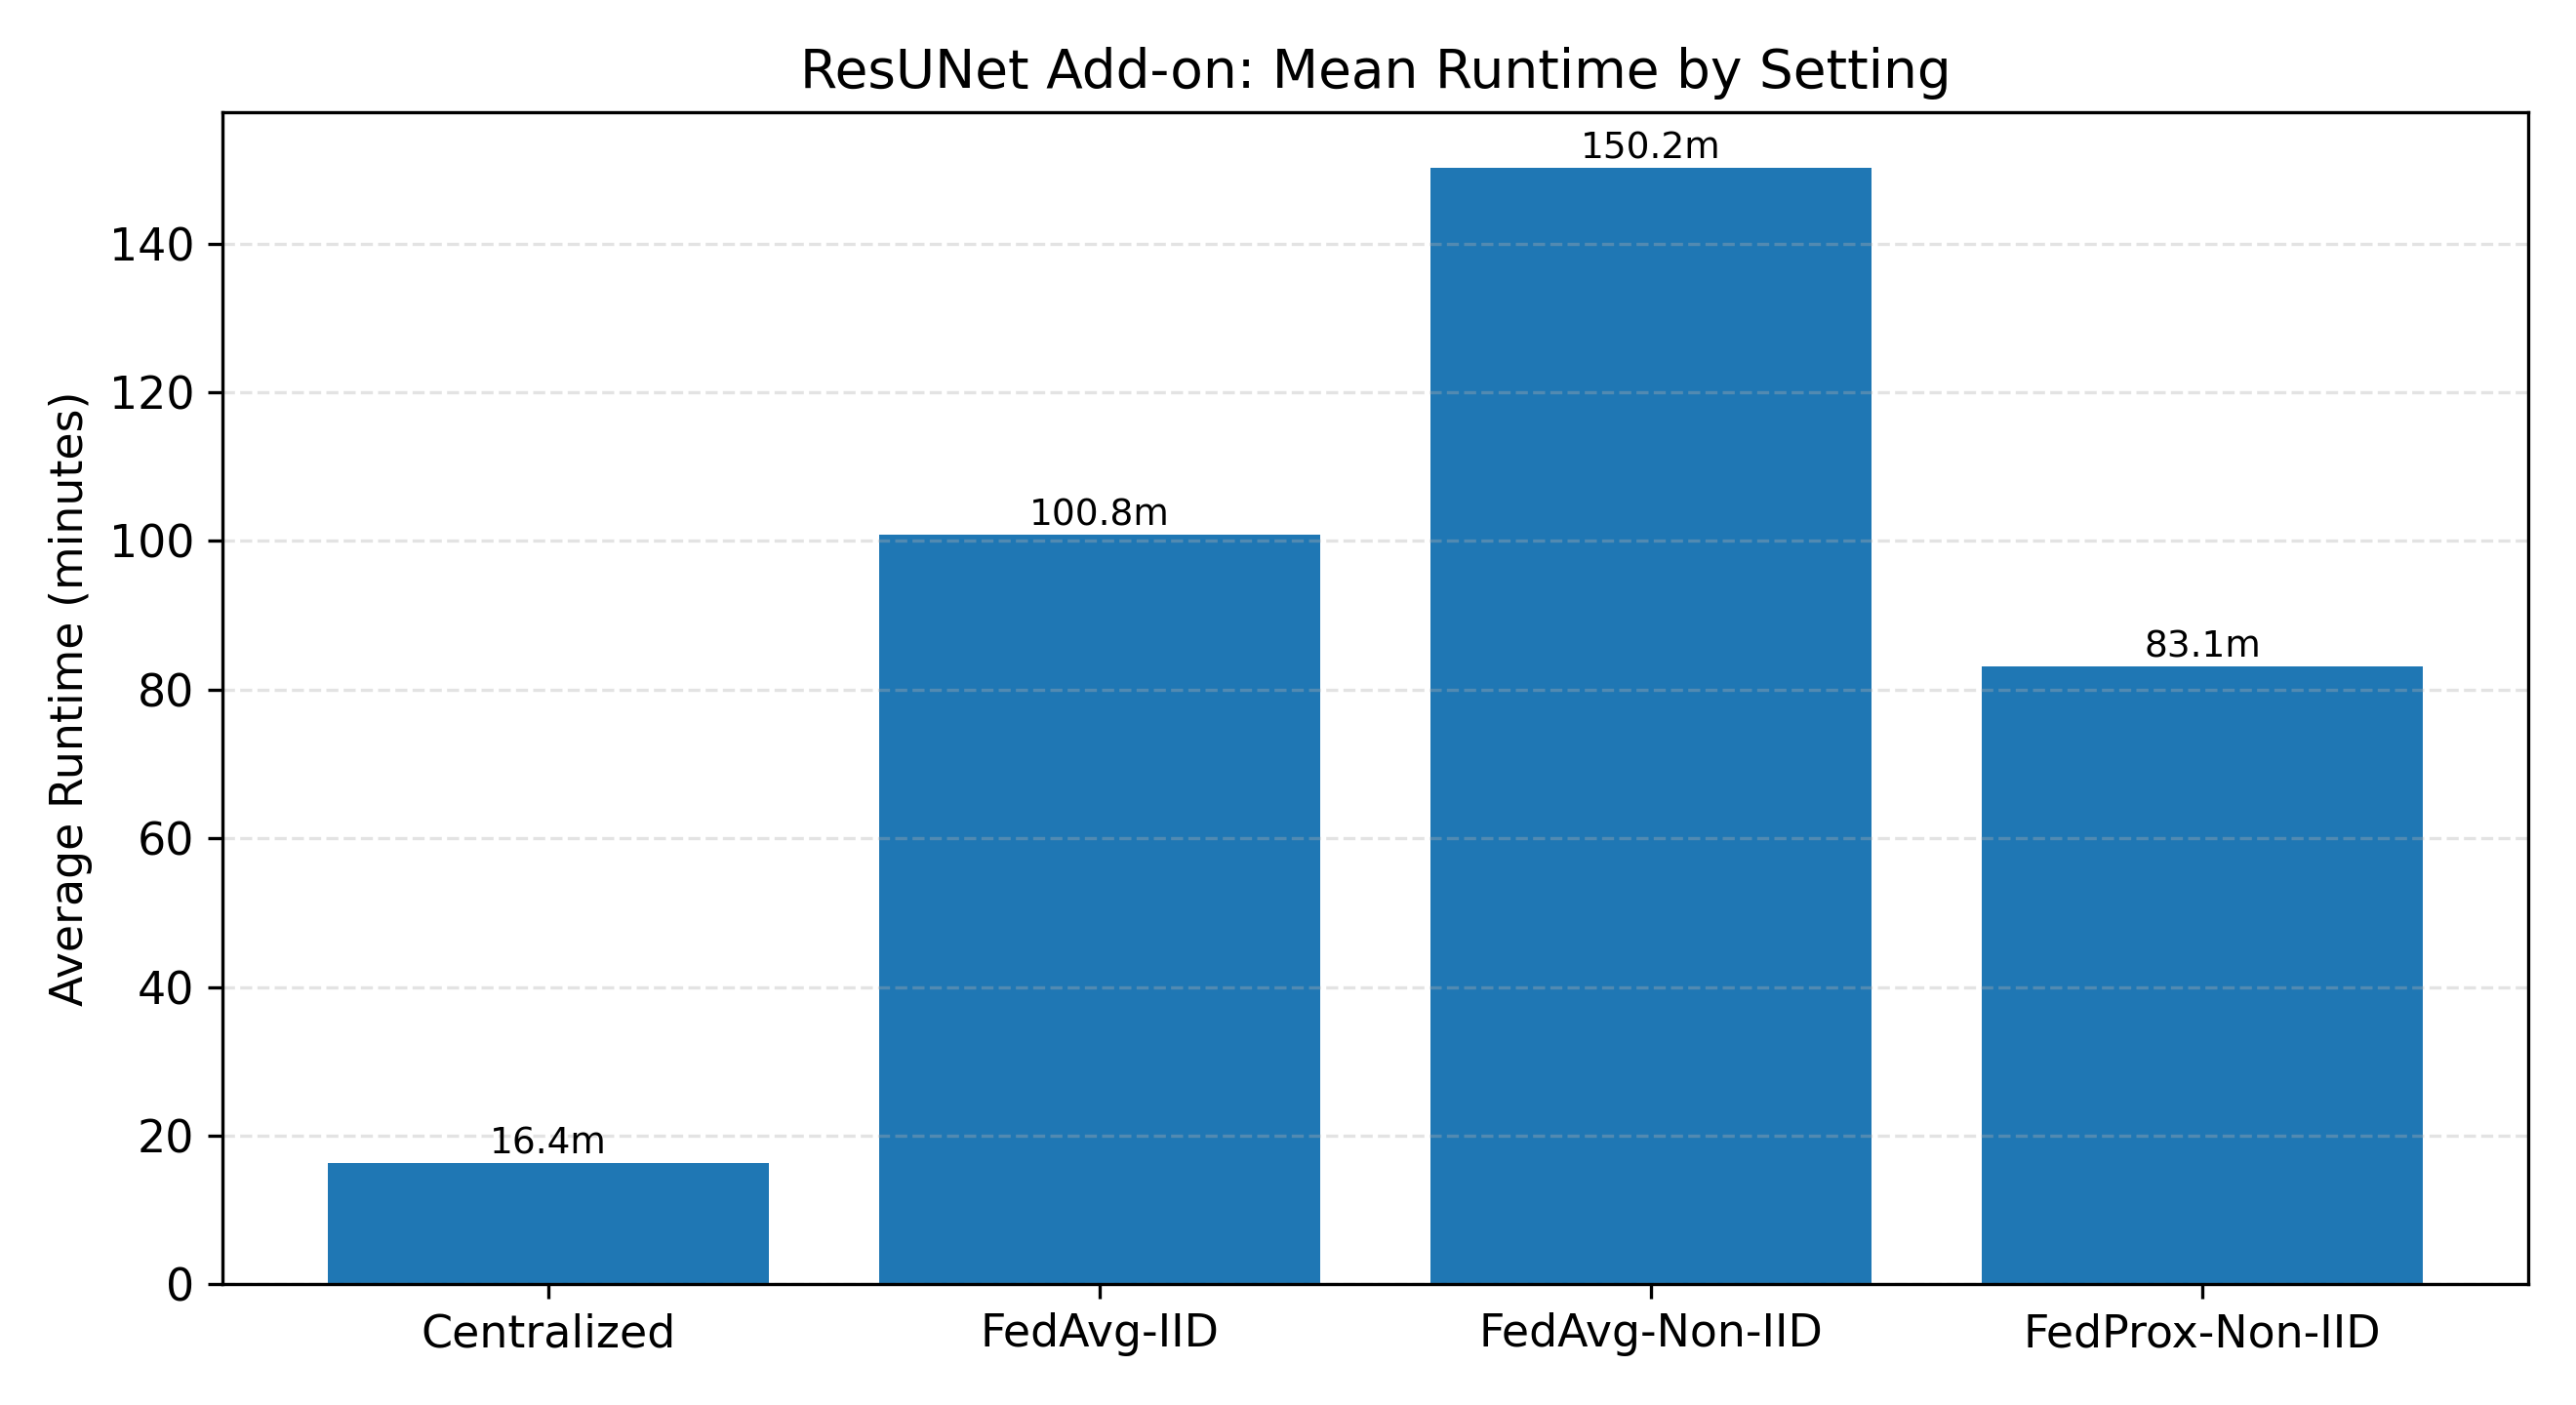
\includegraphics[width=\columnwidth]{results/figures/paper/resunet_addon_runtime_bar.png}
\caption{Supplementary S8: ResUNet runtime profile. Supports systems-level resource discussion.}
\label{fig:s8}
\end{figure}

\begin{thebibliography}{99}

\bibitem{mcmahan2017fedavg}
H. B. McMahan, E. Moore, D. Ramage, S. Hampson, and B. A. y Arcas,
``Communication-efficient learning of deep networks from decentralized data,''
in \emph{Proc. AISTATS}, 2017.

\bibitem{li2020fedprox}
T. Li, A. K. Sahu, M. Zaheer, M. Sanjabi, A. Talwalkar, and V. Smith,
``Federated optimization in heterogeneous networks,''
in \emph{Proc. MLSys}, 2020.

\bibitem{elbir2021flchannel}
A. M. Elbir and S. Coleri,
``Federated learning for channel estimation in conventional and RIS-assisted massive MIMO,''
\emph{IEEE Transactions on Wireless Communications}, 2021.

\bibitem{kairouz2021survey}
P. Kairouz \emph{et al.},
``Advances and open problems in federated learning,''
\emph{Foundations and Trends in Machine Learning}, vol. 14, no. 1--2, pp. 1--210, 2021.

\bibitem{ghosh2019robust}
A. Ghosh, J. Hong, D. Yin, and K. Ramchandran,
``Robust federated learning in a heterogeneous environment,''
arXiv:1906.06629, 2019.

\end{thebibliography}

\end{document}
